% **************************************************
% Document Class Definition
% **************************************************
\pdfobjcompresslevel 0
\documentclass[%
    paper=A4,               % paper size --> A4 is default in Germany
    twoside=true,           % onesite or twoside printing
    openright,              % doublepage cleaning ends up right side
    parskip=full,           % spacing value / method for paragraphs
    chapterprefix=true,     % prefix for chapter marks
    11pt,                   % font size
    headings=normal,        % size of headings
    bibliography=totoc,     % include bib in toc
    listof=totoc,           % include listof entries in toc
    titlepage=on,           % own page for each title page
    captions=tableabove,    % display table captions above the float env
    draft=false,            % value for draft version
    openany					% Avoid blank page after each new part, chapter, ...
]{scrreprt}%


% **************************************************
% Setup thesis document in this file
% **************************************************
%%%%%%%%%%%%%%%%%%%%%%%%%%%%%%%%%%%%%%%%%
% Thesis Configuration File
%
% Important note:
% The main lines to change in this file are in the DOCUMENT VARIABLES
% section, the rest of the file is for advanced configuration.
%
%%%%%%%%%%%%%%%%%%%%%%%%%%%%%%%%%%%%%%%%%
% !TEX root = my-thesis.tex


% **************************************************
% Files' Character Encoding
% **************************************************
\PassOptionsToPackage{utf8}{inputenc}
\usepackage{inputenc}

% **************************************************
% Silence annoying warnings
% **************************************************
\RequirePackage{silence}
\WarningFilter{titlesec}{Non standard sectioning command}
\WarningFilter{scrreprt}{Usage of package}
\WarningFilter{scrreprt}{Activating an ugly workaround}
\WarningFilter{titlesec}{Non standard sectioning command detected}

% **************************************************
% Information and Commands for Reuse
% **************************************************

\newcommand{\thesisTitle}{Exploring the genomic complexity of bacterial infection in 3D}
\newcommand{\thesisName}{Cyril Matthey-Doret}
\newcommand{\thesisSubject}{Thèse de doctorat en Bioinformatique}
\newcommand{\thesisDate}{16 décembre 2021}
\newcommand{\thesisVersion}{0.1}

\newcommand{\thesisPresident}{Angela Taddei}
\newcommand{\thesisPresidentUniversity}{\protect{Sorbonne Université}}
\newcommand{\thesisPresidentDepartment}{UMR 3664 - Nuclear Dynamics, Institut Curie}

\newcommand{\thesisFirstReviewer}{Francesco Ferrari}
\newcommand{\thesisFirstReviewerUniversity}{\protect{IFOM - The FIRC Institute of Molecular Oncology}}
\newcommand{\thesisFirstReviewerDepartment}{Computational Genomics}

\newcommand{\thesisSecondReviewer}{Matthieu Legendre}
\newcommand{\thesisSecondReviewerUniversity}{\protect{Aix Marseille Université}}
\newcommand{\thesisSecondReviewerDepartment}{UMR 7256 - Laboratoire Information Génomique et structurale, Institut de Microbiologie de la Méditerranée}

\newcommand{\thesisSecondExaminer}{Olivier Espeli}
\newcommand{\thesisSecondExaminerUniversity}{\protect{Collège de France}}
\newcommand{\thesisSecondExaminerDepartment}{Center for Interdisciplinary Research in Biology}

\newcommand{\thesisFirstExaminer}{Matthias Horn}
\newcommand{\thesisFirstExaminerUniversity}{\protect{University of Vienna}}
\newcommand{\thesisFirstExaminerDepartment}{Department of Microbiology and Ecosystem Science}


\newcommand{\thesisFirstSupervisor}{Romain Koszul}
%\newcommand{\thesisSecondSupervisor}{Dr. D}

\newcommand{\thesisUniversity}{\protect{Sorbonne Université}}
\newcommand{\thesisUniversityDepartment}{École doctorale Complexité du Vivant}
\newcommand{\thesisUniversityInstitute}{Institut Pasteur}
\newcommand{\thesisUniversityGroup}{Unité de Régulation Spatiale des Génomes}
\newcommand{\thesisUniversityCity}{Paris}
\newcommand{\thesisUniversityCityCedex}{Cedex 15}
\newcommand{\thesisUniversityStreetAddress}{25-28 Rue du Docteur Roux}
\newcommand{\thesisUniversityPostalCode}{75724}


% **************************************************
% Debug LaTeX Information
% **************************************************
%\listfiles


% **************************************************
% Packages options
% **************************************************

\PassOptionsToPackage{% setup clean thesis style
    figuresep=colon,%
    sansserif=false,%
    hangfigurecaption=false,%
    hangsection=true,%
    hangsubsection=true,%
    colorize=full,%
    colortheme=blueroyalred,%
    bibsys=bibtex,%
%     bibfile=Mendeley,%
    bibfile=library,%
    bibstyle=numeric,%
    wrapfooter=true,%
}{cleanthesis}

\PassOptionsToPackage{
	acronyms,
    translate=babel,
    xindy,
    toc,
    nopostdot,
    entrycounter,
    nohypertypes={acronym,notation},
    indexonlyfirst
}{glossaries}

\PassOptionsToPackage{
	english,
	french,
    main=english
}{babel}

\PassOptionsToPackage{
	user,
    counter,
    hyperref
}{zref}

\PassOptionsToPackage{
	nameinlink
}{cleveref}

\PassOptionsToPackage{
	para,
    online,
    flushleft
}{threeparttable}

% Remove several fields in bibliography



% **************************************************
% Load and Configure Packages
% **************************************************


\usepackage{algorithm}
\usepackage{algorithmic}
\usepackage{babel} 						% babel system, adjust the language of the content
\usepackage{cleanthesis}
\usepackage{glossaries}						% Allow glossary and acronyms
%\usepackage[amssymb]{SIunits}				% symboles unites SI (superseded by siunitx)
\usepackage{siunitx}
\usepackage{upgreek,textcomp}               % Non-italic greek characters
\usepackage{chngcntr}						% Reset Chapter counter for each part
\usepackage{amsmath}
%\usepackage[euler]{textgreek}				% For better greek letters in text mode
\usepackage{subcaption}						% Allow subfigures
% \usepackage[lofdepth,lotdepth]{subfig}
% \usepackage{etoolbox}
% \usepackage{zref}							% Better label tags
% \usepackage{cleveref}						% Better autorefs
% \usepackage{xparse}
\usepackage{CJKutf8}
\usepackage{pdfpages}
\usepackage{xassoccnt}
\usepackage[user,counter]{zref}
\usepackage{xparse}
\usepackage{threeparttable}
\usepackage{booktabs}
\usepackage{tabularx}
\usepackage{colortbl}
\usepackage{tabularx}
\usepackage{multirow}
\usepackage{listings}
\usepackage{wrapfig}
\usepackage{array}
\usepackage{placeins}
% \usepackage{nameref}
\usepackage{marginnote}
%\usepackage[utf8]{inputenc}
\usepackage{textgreek}
%\usepackage{minted}

\usepackage{tikz}

\usetikzlibrary{shapes,positioning,arrows}

% **************************************************
% Setup
% **************************************************
% ..................................................
% Commands
% ..................................................
\newsavebox{\largestimage}

\DeclareCiteCommand{\citeauthorfirstlast}
  {\boolfalse{citetracker}%
   \boolfalse{pagetracker}%
   \DeclareNameAlias{labelname}{first-last}%
   \usebibmacro{prenote}}
  {\ifciteindex
     {\indexnames{labelname}}
     {}%
   \printnames{labelname}}
  {\multicitedelim}
  {\usebibmacro{postnote}}
% ref commands, e.g. for images, tables and text labels
% --------------------------------------------------
% RESULT = (siehe Tab. 12.4)
\newcommand{\tabref}[1]{(see Tab.~\ref{#1})}
%
% RESULT = (siehe Tab. 12.4)
\newcommand{\tableref}[1]{(see Tab.~\ref{#1} Page~\pageref{#1})}
%
% --------------------------------------------------
% RESULT = (siehe 3.4)
\newcommand{\tref}[1]{(see \ref{#1})}
%
% RESULT = Abschnitt 3.4
\newcommand{\treft}[1]{Section~\ref{#1}}
%
% RESULT = (siehe 3.4, Seite 12)
\newcommand{\textref}[1]{(see \ref{#1}, Page~\pageref{#1})}
%
% RESULT = Abschnitt 3.4 (siehe Seite 12)
\newcommand{\textreft}[1]{Section~\ref{#1} (see Page~\pageref{#1})}
%
% --------------------------------------------------
% RESULT = (siehe Abb. 10.4)
\newcommand{\fref}[1]{(see Fig.~\ref{#1})}
%
% RESULT = (siehe Abb. 10.4 b)
\newcommand{\frefadd}[2]{(see Fig.~\ref{#1}~#2)}
%
% RESULT = (siehe Abb. 10.4, Seite 12)
\newcommand{\figref}[1]{(see Fig.~\ref{#1}, Page~\pageref{#1})}
%
% RESULT = (siehe Abb. 10.4 b, Seite 12)
\newcommand{\figrefadd}[2]{(see Fig.~\ref{#1}~#2, Page~\pageref{#1})}
%
% RESULT = Abbildung 10.4
\newcommand{\figreft}[1]{Figure~\ref{#1}}
%
% RESULT = Abbildung 10.4 b
\newcommand{\figrefaddt}[2]{Figure~\ref{#1}~#2}
%
% --------------------------------------------------
% RESULT = (siehe Seite 12)
\newcommand{\seepage}[1]{(see Page~\pageref{#1})}
% ..................................................
% Hyperref
% ..................................................
\hypersetup{% setup the hyperref-package options
    pdftitle={\thesisTitle},    %   - title (PDF meta)
    pdfsubject={\thesisSubject},%   - subject (PDF meta)
    pdfauthor={\thesisName},    %   - author (PDF meta)
    plainpages=false,           %   -
    colorlinks=true,            %   - colorize links?
    linktocpage=true,
    pdfborder={0 0 0},          %   -
    breaklinks=true,            %   - allow line break inside links
    bookmarksnumbered=true,     %
    bookmarksopen=true,         %
    linkcolor=ctcolorblue,
    urlcolor=ctcolorblue,
    citecolor=black,
}


% ..................................................
% Counter labels
% ..................................................
\counterwithin*{chapter}{part}	% Reset chapter counter each time part counter is called
\counterwithin{table}{part}
\counterwithout{table}{chapter}
\counterwithin{figure}{part}
\counterwithout{figure}{chapter}
\renewcommand{\thetable}{\thepart.\Alph{table}}
\renewcommand{\thefigure}{\thepart.\Alph{figure}}
\renewcommand*{\figureformat}{\figurename~\thefigure}
\renewcommand*{\tableformat}{\tablename~\thetable}
% ..................................................
% Lists
% ..................................................
%\frenchbsetup{StandardLists=true}
\setlist[itemize]{label={\LARGE\raisebox{-0.3ex}{\textbullet}}, font=\color{ctcoloroyalblue}}
\newlist{todolist}{itemize}{3}
\setlist[todolist]{label={\LARGE\raisebox{-0.3ex}{\textbullet}},font=\color{color_todo}\bfseries,itemsep=0pt,parsep=0pt,before=\color{color_todo}}
% ..................................................
% Glossaries  
% ..................................................
\DeclareDocumentCommand{\newdualentry}{ O{} O{} m m m m } {
  \newglossaryentry{gls-#3}{name={#5},text={#5\glsadd{#3}},
    description={#6},#1
  }
  \makeglossaries
  \newacronym[see={[Glossary:]{gls-#3}},#2]{#3}{#4}{#5\glsadd{gls-#3}}
}
\defglsentryfmt{%
  \ifglsused{\glslabel}{%
    \glsgenentryfmt\ignorespaces%
  }{%
    % Typeset first use
    \textit{\glsgenentryfmt}\ignorespaces%
  }%
}
\renewcommand*{\glsentrycounterlabel}{}%
% \renewcommand*{\glspostlinkhook}{\textsuperscript{\ref{glsentry-\glslabel}}}
% \renewcommand*{\glspostlinkhook}{\textsuperscript{\glsrefentry{\glslabel}}}
% \renewcommand*{\glstextformat}[1]{\textcolor{black}{#1}}		% Hack to remove color links in glossaries
\renewcommand{\glossarypreamble}{\glsresetentrycounter} 
\newglossary[nlg]{notation}{not}{ntn}{Notation}
% \defglsdisplayfirst[\glsdefaulttype]{\textit{#1}\ignorespaces}

% ..................................................
% Bibliography
% ..................................................
\defbibheading{bibliography}[\bibname]{\chapter*{#1}\markboth{#1}{#1}}	% Redefine heading/footer for bibliography

% ..................................................
% Subcaption
% ..................................................
\renewcommand{\thesubfigure}{\alph{subfigure}}
\captionsetup[subfigure]{labelformat=simple, labelsep=none, justification=centering}
% \DeclareCaptionLabelFormat{graysf}{\textcolor{gray}{\sffamily (#2)}}
% \captionsetup[subfigure]{labelsep=space,labelformat=graysf}
% ..................................................
% Caption names
% ..................................................
\renewcaptionname{english}{\figurename}{Fig.}
\renewcaptionname{english}{\tablename}{Tab.}
%\renewcaptionname{french}{\partname}{Partie}
%\renewcaptionname{french}{\tablename}{Tableau}
% ..................................................
% Zref 
% ..................................................
% TODO: Sounds good, doesn't work !!
\makeatletter

% Define new properties
\zref@newprop{childcountervalue}{\arabic{\LastRefSteppedCounter}}% This is the naked value
\zref@newprop{parentcountervalue}{\csname the\GetParentCounter{\LastRefSteppedCounter}\endcsname}
\newenvironment{conditions}
{\par\vspace{\abovedisplayskip}\noindent\begin{tabular}{>{$}l<{$} @{${}={}$} l}}
	{\end{tabular}\par\vspace{\belowdisplayskip}}
% Add the new properties to the main property list stored with \zlabel
\zref@addprops{main}{childcountervalue,parentcountervalue}


\NewDocumentCommand{\parentref}{m}{%
  \zref@ifrefundefined{#1}{%
    -100%
  }{%
    \zref@extract{#1}{parentcountervalue}%
  }%
}


\makeatother

% \GetAllResetLists% Important
% \RegisterPostLabelHook{\zlabel}% Important

% ..................................................
% Color tables 
% ..................................................
% Wener post (https://tex.stackexchange.com/a/33761)
% David Carlisle post at tex.exchange (https://tex.stackexchange.com/a/91498)
\colorlet{blcolor}{gray!80}
\colorlet{tableheadcolor}{gray!25} % Table header colour = 25% gray
\colorlet{tablerowcolor}{gray!10} % Table row separator colour = 10% gray
\newcommand{\headcol}{\rowcolor{tableheadcolor}} %
\newcommand{\rowcol}{\rowcolor{tablerowcolor}} %
% Command \topline consists of a (slightly modified) \toprule followed by a \heavyrule rule of colour tableheadcolor (hence, 2 separate rules)
\newcommand{\topline}{\arrayrulecolor{black}\specialrule{0.1em}{\abovetopsep}{0pt}%
            \arrayrulecolor{tableheadcolor}\specialrule{\belowrulesep}{0pt}{0pt}%
            \arrayrulecolor{black}}
% Command \midline consists of 3 rules (top colour tableheadcolor, middle colour black, bottom colour white)
\newcommand{\midline}{\arrayrulecolor{tableheadcolor}\specialrule{\aboverulesep}{0pt}{0pt}%
            \arrayrulecolor{black}\specialrule{\lightrulewidth}{0pt}{0pt}%
            \arrayrulecolor{white}\specialrule{\belowrulesep}{0pt}{0pt}%
            \arrayrulecolor{black}}
% Command \rowmidlinecw consists of 3 rules (top colour tablerowcolor, middle colour black, bottom colour white)
\newcommand{\rowmidlinecw}{\arrayrulecolor{tablerowcolor}\specialrule{\aboverulesep}{0pt}{0pt}%
            \arrayrulecolor{black}\specialrule{\lightrulewidth}{0pt}{0pt}%
            \arrayrulecolor{white}\specialrule{\belowrulesep}{0pt}{0pt}%
            \arrayrulecolor{black}}
% Command \rowmidlinewc consists of 3 rules (top colour white, middle colour black, bottom colour tablerowcolor)
\newcommand{\rowmidlinewc}{\arrayrulecolor{white}\specialrule{\aboverulesep}{0pt}{0pt}%
            \arrayrulecolor{black}\specialrule{\lightrulewidth}{0pt}{0pt}%
            \arrayrulecolor{tablerowcolor}\specialrule{\belowrulesep}{0pt}{0pt}%
            \arrayrulecolor{black}}
% Command \rowmidlinew consists of 1 white rule
\newcommand{\rowmidlinew}{\arrayrulecolor{white}\specialrule{\aboverulesep}{0pt}{0pt}%
            \arrayrulecolor{black}}
% Command \rowmidlinec consists of 1 tablerowcolor rule
\newcommand{\rowmidlinec}{\arrayrulecolor{tablerowcolor}\specialrule{\aboverulesep}{0pt}{0pt}%
            \arrayrulecolor{black}}
% Command \bottomline consists of 2 rules (top colour
\newcommand{\bottomline}{\arrayrulecolor{white}\specialrule{\aboverulesep}{0pt}{0pt}%
            \arrayrulecolor{black}\specialrule{\heavyrulewidth}{0pt}{\belowbottomsep}}%
\newcommand{\bottomlinec}{\arrayrulecolor{tablerowcolor}\specialrule{\aboverulesep}{0pt}{0pt}%
            \arrayrulecolor{black}\specialrule{\heavyrulewidth}{0pt}{\belowbottomsep}}%
% Middle line connecting heading row and the second row
\newcommand{\rowmidlineHR}{\arrayrulecolor{tableheadcolor}
  \specialrule{\aboverulesep}{0pt}{0pt}%
  \arrayrulecolor{black}\specialrule{\lightrulewidth}{0pt}{0pt}%
  \arrayrulecolor{tablerowcolor}\specialrule{\belowrulesep}{0pt}{0pt}%
  \arrayrulecolor{black}}
  % Command \rowmidlinewc consists of 3 rules
  % (top colour tableheadcolor, middle colour black, bottom colour tablerowcolor)
% Secondary gray middle line 
\newcommand{\rowmidlineG}{\arrayrulecolor{tablerowcolor}%
  \specialrule{\aboverulesep}{0pt}{0pt}%
  \arrayrulecolor{blcolor}\specialrule{\lightrulewidth}{0pt}{0pt}%
  \arrayrulecolor{tablerowcolor}\specialrule{\belowrulesep}{0pt}{0pt}%
  \arrayrulecolor{black}}
\renewcommand{\arraystretch}{1.3}
\newcolumntype{Y}{>{\centering\arraybackslash}X}
\newcolumntype{C}{>{\centering\arraybackslash}c}
\newcolumntype{M}{>{\centering\arraybackslash}m}
% ..................................................
% Listings
% ..................................................
\lstdefinelanguage{Ini}
{
	basicstyle=\ttfamily\small,
	columns=fullflexible,
	morecomment=[s][\color{Orchid}\bfseries]{[}{]},
	morecomment=[l]{\#},
	morecomment=[l]{;},
	commentstyle=\color{gray}\ttfamily,
	morekeywords={},
	otherkeywords={=,:},
	keywordstyle={\color{green}\bfseries}
}


%\newenvironment{conditions}
%{\par\vspace{\abovedisplayskip}\noindent\begin{tabular}{>{$}l<{$} @{${}={}$} l}}
%	{\end{tabular}\par\vspace{\belowdisplayskip}}


% **************************************************
% Compute glossary index
% **************************************************
%----------------------------------------------------------------------------------------
%	Glossary
%----------------------------------------------------------------------------------------

\newglossaryentry{gloss}{
	name={Glossary entry},
	text={Glossary entry text},
	description={Glossary entry description}
}


%----------------------------------------------------------------------------------------
%	Notations
%----------------------------------------------------------------------------------------

\newglossaryentry{angstrom}
{
	type=notation,
	name={Angstr\" om (\angstrom)},
    text=Angstr\" om,
	description={Unité de mesure valant 0.1 nm (10\textsuperscript{- 10} m)},
	sort={angstrom}
}

\newglossaryentry{parthenogenesis}
{
		name={parthenogenesis},
		description={Mode of reproduction where females generate offspring asexually.}
}

\newglossaryentry{chromatin}
{
		name={chromatin},
		description={An association of DNA and various DNA-binding proteins forming chromosomes.}
}

\newglossaryentry{contig}
{
	name={contig},
	description={Contiguous subsequence of a DNA molecule generated by combining multiple reads.}
}

\newglossaryentry{euchromatin}
{
		name={euchromatin},
		description={The active portion of chromatin}
}

\newglossaryentry{fitness}
{
		name={fitness},
		description={The reproductive success of an organism or individual.  It is equal to the average contribution to the gene pool of the next generation of the population.}
}

\newglossaryentry{heterochromatin}
{
		name={heterochromatin},
		description={The inactive portion of chromatin}
}

\newglossaryentry{Muller}
{
		name={Muller's ratchet},
		description={The irreversible accumulation of slightly deleterious mutations in genomes with lack of recombination.}
}

\newglossaryentry{polishing}
{
	name={polishing},
	description={The use of short accurate reads to correct a genome assembly generated with error prone long reads.}
}

\newglossaryentry{read}
{
	name={read},
	description={Contiguous subsequence of a DNA molecule as read by a sequencing technology.}
}

\newglossaryentry{restriction enzyme}
{
	name={restriction enzyme},
	description={Protein that cleaves DNA at specific recognition sites.}
}

\newglossaryentry{scaffold}
{
	name={scaffold},
	description={Discontinuous subsequence of a DNA molecule generated by combining multiple contigs.}
}


%----------------------------------------------------------------------------------------

%	Acronyms
%----------------------------------------------------------------------------------------
\newacronym{3C}{3C}{Chromosome Conformation Capture}
\newacronym{BAC}{BAC}{Bacterial Artificial Chromosome}
\newacronym{ChIPseq}{ChIPseq}{Chromatin Immuno-Precipitation Sequencing}
\newacronym{CTCF}{CTCF}{CCCTC-binding binding factor}
\newacronym{HGT}{HGT}{Horizontal Gene Transfer}
\newacronym{LCV}{LCV}{\textit{Legionella} Containing Vacuole}
\newacronym{NGS}{NGS}{Next Generation Sequencing}
\newacronym{PFGE}{PFGE}{Pulsed Field Electrophoresis Gel}
\newacronym{RFLP}{RFLP}{Restriction Fragment Length Polymorphism}
\newacronym{SCV}{SCV}{\textit{Salmonella} Containing Vacuole}
\newacronym{SMC}{SMC}{Structural Maintenance of Chromosomes}
\newacronym{TAD}{TAD}{Topologically Asscociating Domain}
\newacronym{WGS}{WGS}{Whole Genome Sequencing}

%----------------------------------------------------------------------------------------
%	Dual entries
%----------------------------------------------------------------------------------------
\newdualentry{SV} % label
	{SV}            % abbreviation
 	{Structural variant}  % long form
 	{Large scale alterations in a genome, including deletions, insertions and insertions} % description

\newdualentry{SNP}
	{SNP}
	{Single Nucleotide Polymorphism}
	{Punctual mutations in a DNA sequence consisting of a nucleotide substitution.}

\newdualentry{indel}
	{indel}
	{Insertion / Deletion}
	{Short mutations in a DNA sequence consisting of a few added or missing nucleotides.}

\makeglossaries
\glsdisablehyper 	% Disable hyper links with glossary entries

% **************************************************
% Document CONTENT
% **************************************************
\begin{document}

% --------------------------
% rename document parts
% --------------------------


% --------------------------
% Front matter
% --------------------------
\pagenumbering{roman}			% roman page numbing (invisible for empty page style)
\pagestyle{empty}				

% \input{examples/titlepages}		% INCLUDE: all titlepages
% !TEX root = ../my-thesis.tex
%
% % ------------------------------------  --> cover title page
%\begin{titlepage}
%	\pdfbookmark[0]{Couverture}{Cover}
%	\flushright
%	\hfill
%	\vfill
%	{\LARGE\thesisTitle \par}
%	\rule[5pt]{\textwidth}{.4pt} \par
%	{\Large\thesisName}
%	\vfill
%	\textit{\large\thesisDate} \\
%	Version: \thesisVersion
%\end{titlepage}
%

% ------------------------------------  --> main title page
\begin{titlepage}
	\thispagestyle{fancytitlepage}
	\pdfbookmark[0]{Titre}{Titlepage}
	\tgherosfont
	\centering

	{\Huge \thesisUniversity} \\[2mm]
    {\Large \thesisUniversityDepartment} \\[2mm]
	
\includegraphics[width=8cm]{FrontBackMatter/gfx/UPMC_Sorbonne_Universites_Logo} \\[2mm]	
	\textsf{\large \thesisUniversityGroup} \\
    \textsf{\large \thesisUniversityInstitute} \\

	\vfill
	{\large \thesisSubject} \\[10mm]
	{\LARGE \color{ctcolortitle}\textbf{\thesisTitle} \\[10mm]}
	{\Large \thesisName} \\[5mm]
    {\Large Directeur de thèse: \textbf{\thesisFirstSupervisor}}\\
    {\Large Co encadrant de thèse: \textbf{\thesisSecondSupervisor}}\\
    \vfill
    
    {\large Présentée et soutenue publiquement le \thesisDate }\\[5mm]
    {\large Jury}\\
	\begin{tabular}{>{\Large\bfseries}l>{\Large}l}
		\thesisPresident~(PU) & Président\\
        \thesisFirstReviewer~(DR) & Rapporteur\\
        \thesisSecondReviewer~(MCU) & Rapporteur\\
        \thesisFirstExaminer~(CR) & Examinateur\\
        \thesisFirstSupervisor~(PR) & Examinateur\\
        \thesisSecondSupervisor~(CR) & Examinateur\\
	\end{tabular}
\end{titlepage}


% ------------------------------------  --> lower title back for single page layout
\hfill
\vfill
{
	\small
	\textit{\thesisTitle} \\
    \thesisName\ \textcopyright\ \thesisDate \\
	\thesisSubject\\
	Rapporteurs: \thesisFirstReviewer\ et \thesisSecondReviewer \\
    Examinatrice: \thesisFirstExaminer\\\
	Directeur de th\`ese: \thesisFirstSupervisor\\
    Co-Directeur de th\`ese: \thesisSecondSupervisor \\[1.5em]
	\textbf{\thesisUniversity} \\
    \thesisUniversityDepartment \\[1.5em]
    \textbf{\thesisUniversityGroup} \\
	\thesisUniversityInstitute \\
    \thesisUniversityStreetAddress \\
	\thesisUniversityPostalCode\ \thesisUniversityCity~\thesisUniversityCityCedex
}		% INCLUDE: all titlepages

\pagestyle{plain}				% display just page numbers
% \input{examples/abstract}		% INCLUDE: the abstracts (english and german)
% !TEX root = ../thesis-example.tex
%
\pdfbookmark[0]{\abstractname}{abstract}
\chapter*{\abstractname}
\label{sec:abstract}
\vspace*{-10mm}

\blindtext

\vspace*{20mm}

\chapter*{Abstract}
\label{sec:abstract-diff}

\blindtext
		% INCLUDE: the abstracts (english and german)

% \input{examples/acknowledgement} % INCLUDE: acknowledgement
% !TEX root = ../thesis-example.tex
%
\pdfbookmark[0]{Acknowledgements}{Acknowledgements}
\chapter*{Acknowledgements}
\label{sec:acknowledgements}
\vspace*{-10mm}

\blindtext
 % INCLUDE: acknowledgement

%
% Table of Contents - List of Tables/Figures/Listings and Acronyms

\pdfbookmark[0]{\contentsname}{contents} % Bookmark name visible in a PDF viewer
\setcounter{tocdepth}{2}		% define depth of toc
\setcounter{secnumdepth}{2} % Depth of sections to number in the text itself - currently up to subsubsections
\tableofcontents				% display table of contents
\clearpage

%----------------------------------------------------------------------------------------
%	List of Figures
%----------------------------------------------------------------------------------------

\listoffigures
\clearpage

%----------------------------------------------------------------------------------------
%	List of Tables
%----------------------------------------------------------------------------------------

\listoftables
        
\clearpage
    
%----------------------------------------------------------------------------------------
%	List of Listings
%---------------------------------------------------------------------------------------- 

% \refstepcounter{dummy}
%\addcontentsline{toc}{chapter}{\lstlistlistingname} % Uncomment if you would like the list of listings to appear in the table of contents
% \pdfbookmark[1]{\lstlistlistingname}{lol} % Bookmark name visible in a PDF viewer

% \lstlistoflistings 

% \vspace{8ex}
% \newpage
       
%----------------------------------------------------------------------------------------
%	Acronyms
%----------------------------------------------------------------------------------------

% \setglossarystyle{list} 
{\singlespacing
\printglossary[type=\acronymtype,title={Abbreviations}]
}
%----------------------------------------------------------------------------------------
%	Glossary
%----------------------------------------------------------------------------------------

\newpage
% \refstepcounter{dummy}

%\setglossarystyle{altlist} 
\printglossary[title={Glossary}] % Contents, list of figures/tables/listings and acronyms

% --------------------------
% Body matter
% --------------------------
\pagenumbering{arabic}			% arabic page numbering
% \setcounter{page}{1}			% set page counter
\pagestyle{maincontentstyle} 	% fancy header and footer

%------------------------------------------------

%\ctpartquote{\cleanchapterquote{In the drama of life on a molecular scale, proteins are where the action is}{\citeauthorfirstlast{Lesk2001}}{\citetitle{Lesk2001} \citep{Lesk2001}}}

\ctparttext{In this introductory part, we delve into the biology of infection and describe the complex relationships between pathogens and their hosts. We also discuss the evolutionary implications of these associations. We then focus on two model systems for infection biology: \textit{Salmonella enterica} and \textit{Legionella pneumophila}. We then provide an overview of how recent advances in genomics have pushed the knowledge of these systems and their current limitaitons.} % Describe here content of the first part

\part{Introduction} % First part of the thesis

% Chapter X

\chapter{Host parasite interactions} % Chapter title

\label{ch:01-01} % For referencing the chapter elsewhere, use \autoref{ch:name} 


Organisms in all branches of the tree of life establish stable interactions with different species. These are often classified according to their perceived impact on the fitness of their members. We traditionally talk about parasitism for interactions with one-way benefits, and mutualism when the interaction has a positive impact on all parties involved.

Biological interactions are observed at different scales, from nanometer-scale virophages infecting giant viruses to fungi forming mycorrhyzal networks spanning up to several kilometers allowing exchange of nutrients with plants root systems. These interactions shape the evolutionary trajectories of the species involved and their genomic landscapes. These genomic changes can sometimes result in drastic transitions in the organisms' lifestyle. This can be the case for example with intracellular bacteria forming symbiosis with their host cells, known as endosymbionts. Wolbachia is a famous example of endosymbiotic bacteria infecting arthropod species. This bacterium is a reproductive parasite illustrating the sometimes blurry line between parasitism and mutualism. It alters the reproductive capabilities of its host, causing some sexual species to reproduce asexually by parthenogenesis for its own benefit. In some species infection by Wolbachia has even become necessary for reproduction. While the bacterium takes advantage of its host reproduction, it also provides numerous advantages such as resistance to viruses in mosquito species and help with vitamin synthesis in flies.


% These interactions can occur at multiple scales (virophages, giant viruses, bacteria, fungi, plants, animals) example of Wolbachia
\section{The evolutionary context of host parasite interactions}

An analogy often used to describe the evolutionary dynamics of host-parasite interactions is an arms race, where each organism evolves novel strategies to improve its own fitness at the expense of the other. This is the case for intracellular bacteria such as Legionella, which can secrete a large arsenal of effector proteins into their host's cytoplasm. Many of these proteins are redundant in the sense that they interact with the same host proteins or pathways. This redundancy is likely an important strategy for parasites with several hosts or changing environments, as some of those redundant effectors could be functional in different hosts or particular environmental conditions.

As intracellular parasites become reliant on their host for most metabolic pathways, they undergo a process known as genome reduction: Pathways provided by the host need no longer be encoded by the parasite and are therefore lost. This process eventually leads to the parasite becoming completely reliant on its host. The progressive accumulation of mutation (and loss) in their genome is known as Muller's ratchet. The only way for intracellular parasites to escape this ineluctable degradation is to acquire genetic material, either from their host or from other microorganisms sharing the same host cytoplasm.

Such genetic transfers are known as horizontal gene transfer (HGT) and are a major contributor to bacterial genomes, with an estimated 80\% of genes being the product of HGT. More recently, HGT have also been detected in eukaryotes. Although they are much less frequent (about 1\% of genes), gene transfers from intracellular microorganisms to eukaryotic hosts are thought to have been involved in major shifts in environmental niche. Examples are the terrestrial colonization of plants and extremophile eukaryotes such as sea ice diatoms which acquired ice binding proteins from prokaryotes.

\section{Amoeba as a host model}

\section{\textit{Legionella pneumophila}}

\textit{L. pneumophila} infects amoeba in the wild but can also infect humans.

\section{\textit{Salmonella enterica}}

Unlike {L. pneumophila}, {S. enterica} only infects birds and mammals. It is a major human pathogen. % Chapter 1
% Chapter X

\chapter{Infection through the lense of genomics} % Chapter title

\label{ch:01-02} % For referencing the chapter elsewhere, use \autoref{ch:name} 

%----------------------------------------------------------------------------------------

The toolset to detect and investigate bacterial infection traditionally included biochemical assays and microscopy. The recent technological advances in DNA sequencing have spurred a rapid extension of this toolset with NGS-derived methods. Here we introduce the different ways genomics can provide biological insights into the biology of bacterial pathogens.

\section{Pathogen characterization}

The most fundamental task related to infection in biomedical research is to detect the presence of infectious agents and characterize them. This allows to test patients presenting suspicious symptoms for the presence of known pathogens, or determine the pathogenicity of a particular strain. 

Genotyping was traditionally achieved using molecular biology techniques, such as \acrfull{RFLP} or \acrfull{PFGE} \cite{ochoa-diazBacterialGenotypingMethods2018}. These techniques rely on the negative charge of the DNA molecules. When put in a gel submitted to an electromagnetic field, these molecules will migrate along the electrical current. The migration distance is proportional to the size of molecules. After migration is complete, the gel can be treated with chemical markers to highlight the location of DNA molecules. This will reveal discrete bands of similar-length DNA fragments. Together these bands form a bar-code which can be interpreted by the scientist to draw conclusion about the number and size of these fragments. In the case of \acrshort{RFLP}, the genome is prealably digested by \Gls{restriction enzyme}s. The digestion will result in a series of fragments whose lengths can be seen on the gel. Bacterial genotypes wil have different mutations which will affect the digestion pattern and resulting barcode on the gel.

While these methods work well to determine differences between alleles, they do not inform us on the actual DNA sequence involved. The advent of DNA sequencing made it possible to directly link phenotype with associated sequences of nucleotides. \acrfull{WGS} provides accurate information on an organism's genotype, down to down to the \acrfull{SNP}, allowing to define genotypes at a finer scale. The main shortcoming of \acrshort{WGS} is its higher cost than other genotyping techniques, but the recent plummeting of sequencing costs have made it releatively affordable. These advantages have made \acrshort{WGS} a popular approach in clinical settings.

\section{Genomics to probe homeostasis}

When host cells are exposed to or infected by a pathogen, their homeostatic state is disrupted. This disruption is a combination of alterations caused by the pathogen to colonize the host cell and host-triggered immune reactions to improve its survival. These two components can usually be unentangled in infection experiments by using a disabled pathogen. The pathogen will still harbour the antigens triggering host reactions, but will be unable to cause any harms. One can then deduce the pathogen-caused disruptions by comparing the infection results from a standard and disabled pathogen. 

Multiple levels of regulation are affected upon infection, from signalling to epigenetic modifications \cite{rolandoLegionellaPneumophilaType2014}, and over the years, a vast arsenal of NGS techniques have been developed to read these regulatory states. 

The most frequently used feature is gene expression. The transcribed RNAs present in the sample can be reverse-transcribed into cDNA and sequenced and the relative abundance of each gene's transcript allows to quantify the expression of the whole genome, known as the transcriptome. Transcriptomes can then be compared between different conditions to find out which genes undergo perturbations during infection. 

Many levels of regulation allow to fine tune gene expression in eukaryote (Fig. \ref{fig:01-02:transcriptional-regulation}). Regulatory elements can be directly encoded by the sequence and trigger the recruitment of protein complexes to fine tune gene expression. Epigenetic changes, in the form of chemical modification of histone proteins offer yet another way to regulate gene expression in eukaryotes. The amount of these epigenetic marks can be measured along the genome using another NGS-derived technique known as \acrfull{ChIPseq}. In \acrshort{ChIPseq}, the chromatin sample is crosslinked with formaldehyde to generate covalent bonds between proteins and DNA. The sample is then sonicated to break the DNA into smaller fragments. Beads coated with specific antibodies against a protein of interest (e.g. an epigenetic mark) are then added and the beads are then precipitated to retrieve them. The crosslinked is then reversed and the DNA fragments purified. This allows to retrieve all genomic regions that were bound to the protein of interest. 

\begin{figure}
    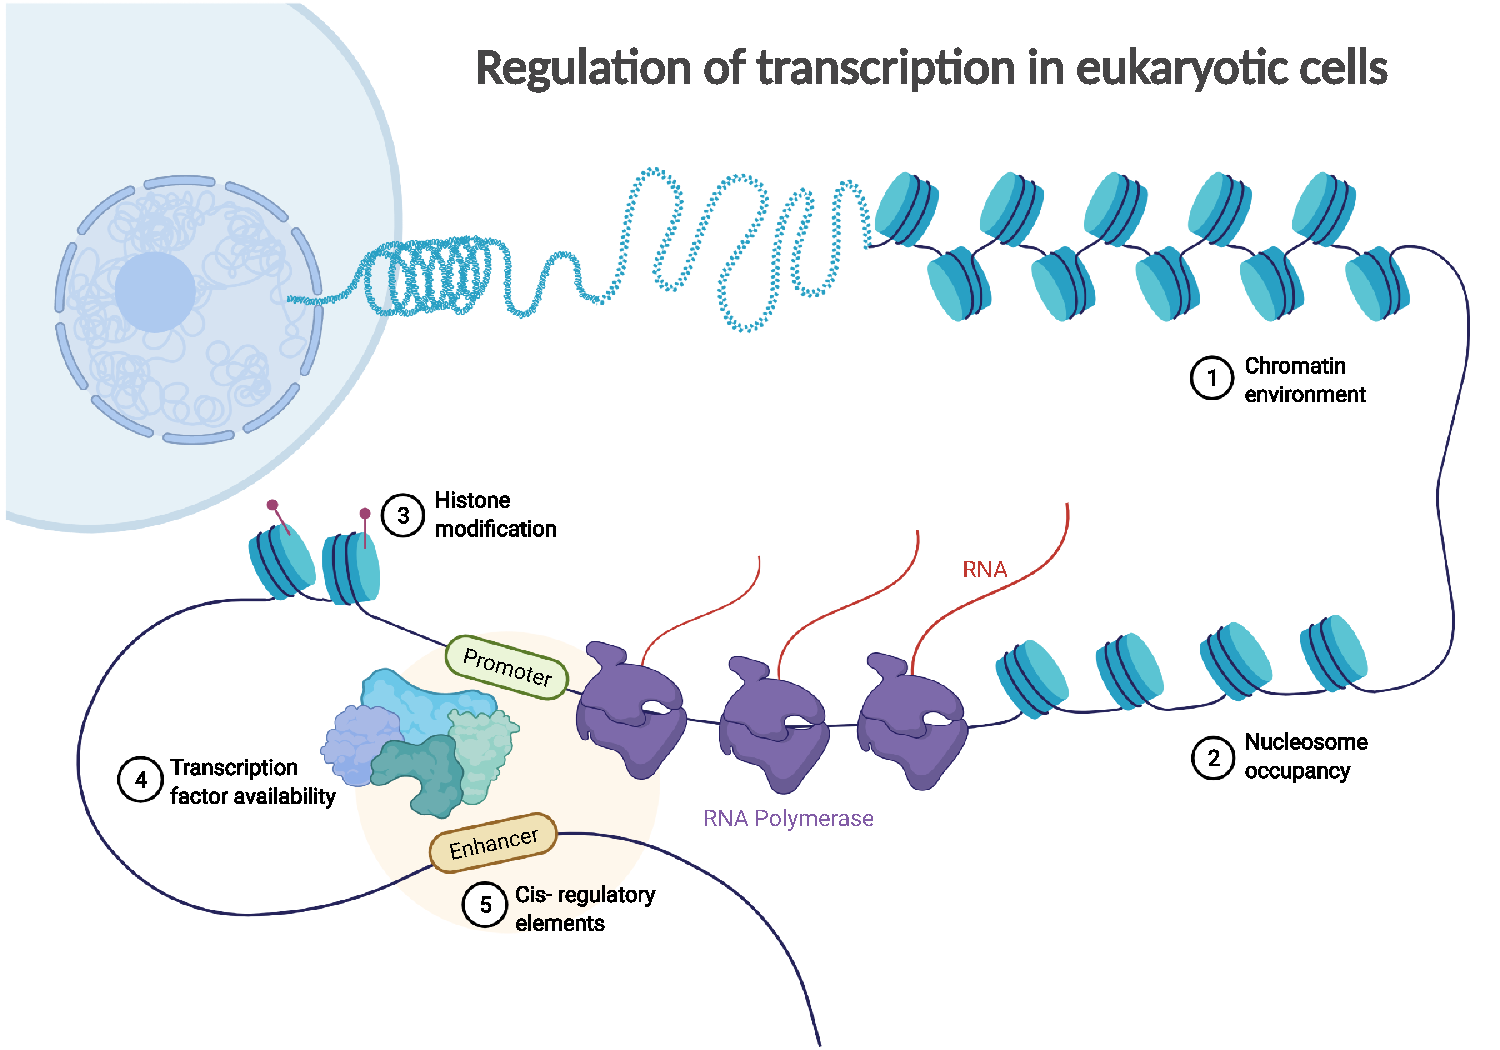
\includegraphics[width=\textwidth]{Parts/Part01/gfx/transcriptional_regulation_levels.pdf}
    \caption{Regulation of transcription in eukaryotic cells. Visual summary of the different levels at which transcription can be regulated. At the largest scale (1), the chromatin environment can form structures affecting transcription. The open space between nucleosome can also affect accessibility of protein complexes to gene sequences (2). Chemical modifications on histone proteins form an epigenetic code defining the recruitment of transcriptional complexes on the genome (3). The availablity of those factors (4) and the proximity of regulatory sequences such as enhancers (5) provide another level of transciptional regulation. Reprinted from “Regulation of Transcription in Eukaryotic Cells”, by BioRender.com (2020). Retrieved from https://app.biorender.com/biorender-templates }
    \label{fig:01-02:transcriptional-regulation}
\end{figure}


\section{Capturing chromosome conformation}

Although DNA is a linear (or circular) molecule, it can fold back on itself and form three-dimensional structures which have several benefits compared to a linear structure. These benefit include compactness: For example, the human chromosome 1 consists of 250 millions nucleotides each spaced by 0.34nm \cite {langridgeMolecularConfigurationDeoxyribonucleic1960}. If straightened, the chromosome would be 85mm long, but the whole genome fits in a nucleus where the diameter is around 10$\mu m$. Another key feature of genome folding is the regulation of gene expression through higher order structures. Compacting large regions of the genome by spreading of \Gls{heterochromatin} allows to downregulate their activity. Smaller scale structures allow to fine tune gene regulation more locally. For example, \Gls{chromatin} loops can bring enhancer and promoters in close spatial proximity even if they would otherwise be far apart on the linear sequence. Compact chromatin domain also form local neighbourhoods where different loci are in close spatial proximity, while loci in distinct domains are isolated from each other. All these levels of spatial regulation are important to understand the coordination of the gene expression programme with other celluar processes.

\subsection{3C technologies}

The use of genomics to investigate the three-dimensional organisation of the genome started with the invention of \acrfull{3C} \cite{dekkerCapturingChromosomeConformation2002}. This technique allowed to measure the frequency of physical interactions a pair of loci (Fig. \ref{fig:01-02:3c}). This is done by crosslinking the genome with formaldehyde, which forms stable bonds between DNA and proteins, and subsequently digesting the genome with a restriction enzyme. Genomic regions closer in space will be crosslinked together more frequently, resulting in pairs or complexes of chromatin fragments from different genomic regions that were spatially interacting. The digested genome is then religated. Loci which are closer in space are religated more often with each other in the population of cells. The crosslink is then reverted and primers from two regions of interest are added to perform qPCR. This allows to measure the quantity of religated products containing the two loci of interest. Thus, 3C allows to quantify the spatial proximity between two known genomic loci.

\begin{figure}[htb]
    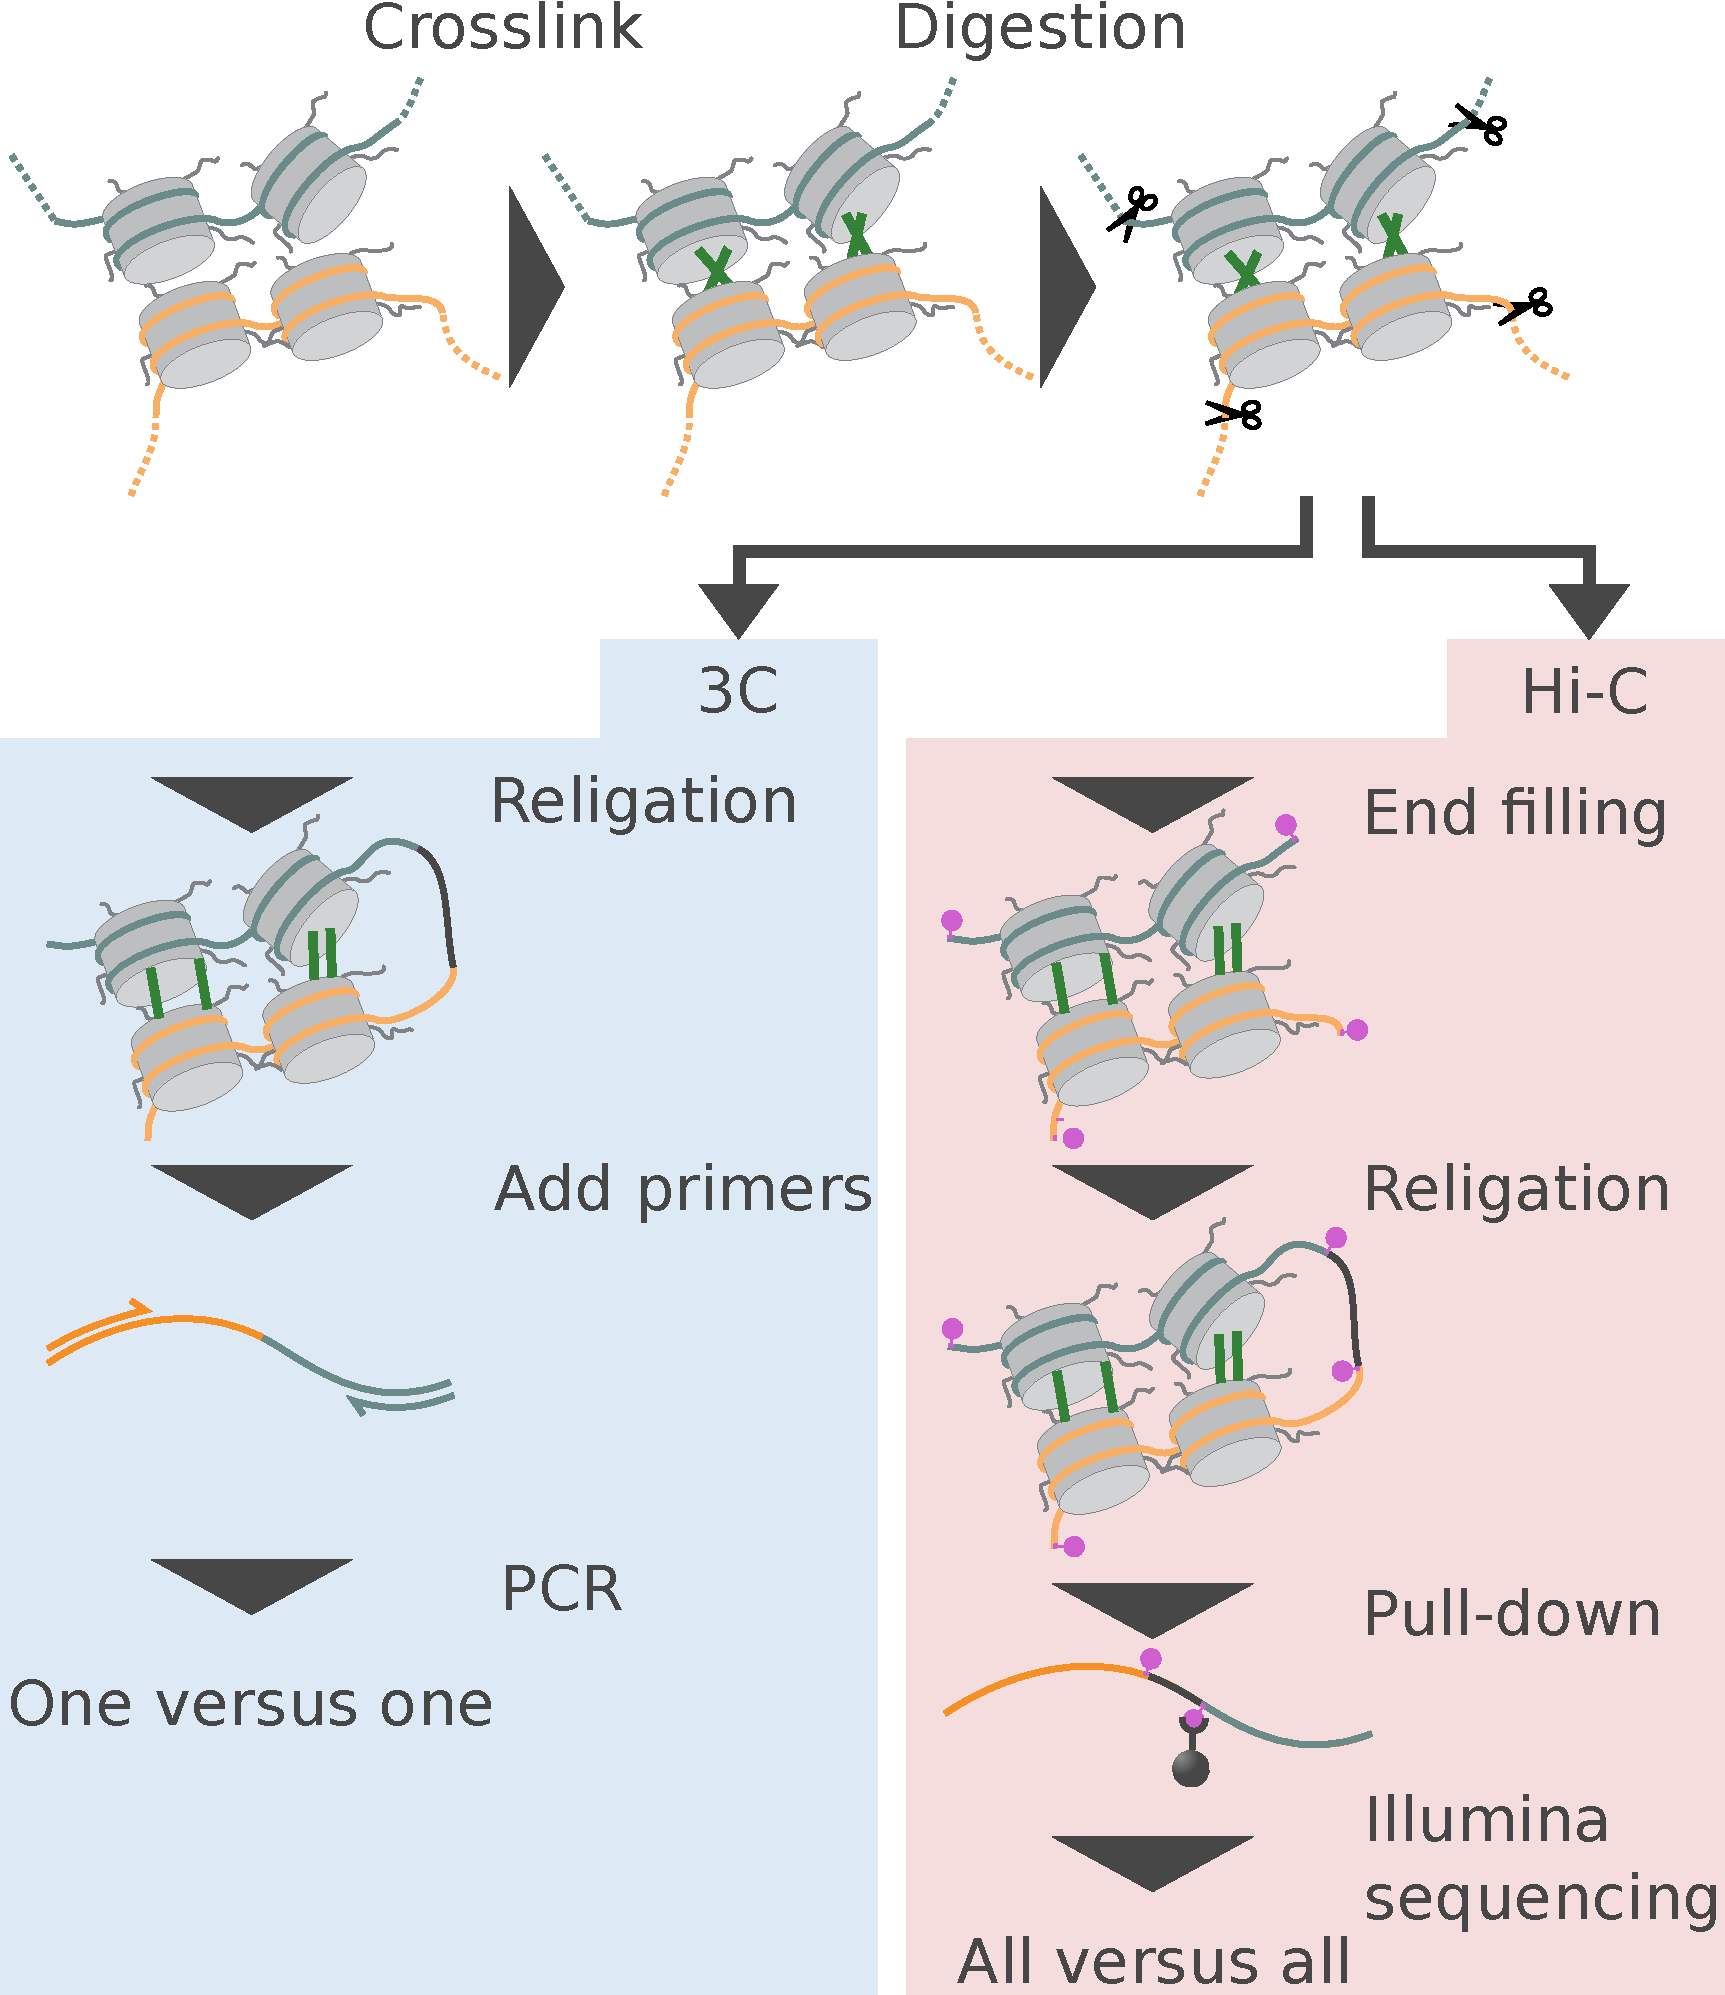
\includegraphics[width=\textwidth]{Parts/Part01/gfx/3c_protocol.pdf}
    \caption{Chromosome conformation capture protocol: Chromosome conformation capture protocol share common steps (top): The chromatin is first crosslinked to form covalent DNA-protein bonds and then digested using a restriction enzyme. The Hi-C protocol subsequently differs from the original 3C protocol. In 3C (left), fragments are religated, the crosslinked is reversed and specific primers are added to amplify a pair of known loci. This allows to quantify interaction between 2 loci. In Hi-C (right), the fragments ends are filled with biotinylated nucleotides (pink), religated and the crosslinked is reversed. Streptavidin beads are then used to pull down religation products which are then sequenced.}
	\label{fig:01-02:3c}
\end{figure}

Since then, many derivatives of the \acrshort{3C} technique have been developed. The most significant improvement was brought by Hi-C (Fig. \ref{fig:01-02:3c}, right). This method shares several steps with 3C, the main difference being that next generation sequencing is used instead of qPCR. This allows to quantify the interaction frequency of all versus all loci in the genome instead of using specific primers for a pair of locus. In Hi-C, fragment ends are filled with biotin prior to religation \cite{lieberman-aidenComprehensiveMappingLongRange2009}. The religation products are then pulled-down using streptavidin beads (which have high affinity for biotin), which allows to specifically retain digested  and religated products for sequencing.

The information generated by Hi-C experiments is a list of contacts between all pairs of restriction fragments in the genome. These contacts are most commonly visualized using contact maps (Fig. \ref{fig:01-02:hic}a), which are two entry tables represented as color-coded matrices. The color of each value in the matrix is proportional to its value and reflects the interaction frequency between the associated pair of fragments. Those contact maps are an indirect representation of the tri-dimensional folding of chromosomes and are rich in information.

The various folding structures formed by chromatin are created by DNA binding proteins. The most common example is the \acrfull{CTCF}, a transcription factor that also acts as an "architectural protein" structuring chromatin. Molecular motors such as cohesin and other \acrfull{SMC} family proteins slide along DNA to operate various roles. When cohesin is loaded onto the chromosome, it can extrude two strands of DNA in opposite directions through it's ring-shaped structure, a process known as loop extrusion \cite{fudenbergFormationChromosomalDomains2016}. When cohesin encounters a roadblock protein such as \acrshort{CTCF} the extrusion stops, forming a chromatin loop and maintaining contact between the two DNA strands. Depending on the location of those roadblocks, this can form stable interactions between distant genomic regions. 

Each spatial structure formed by chromatin is reflected on the contact map as a distinct pattern (Fig. \ref{fig:01-02:hic}b). At the largest scale, chromosomes are isolated from each other in the nucleus, occupying distinct "chromosome territories". This is reflected as dark squares along the diagonal of the whole genome contact map as each chromosome interacts more with itself than any other chromosome (Fig. \ref{fig:01-02:hic}a). Within each chromosome chromatin forms "insulation domains", known as \acrfull{TAD}s in mammals. Genes sharing the same domain are in close proximity, while being isolated from genes in neighbouring domains . Genes within the same domain also tend to be co-regulated \cite{noraSpatialPartitioningRegulatory2012}. Domains form dark squares along the diagonal of a chromosome, due to the enriched intra-domain interactions at the expense of inter-domain contacts (Fig. \ref{fig:01-02:hic}b, bottom). At a finer scale, chromatin loops are visible on contact maps as dots away from the diagonal (Fig. \ref{fig:01-02:hic}b, middle). The coordinates of those dots correspond to the genomic positions of roadblocks which stopped the extrusion process.

\begin{figure}[htb]
    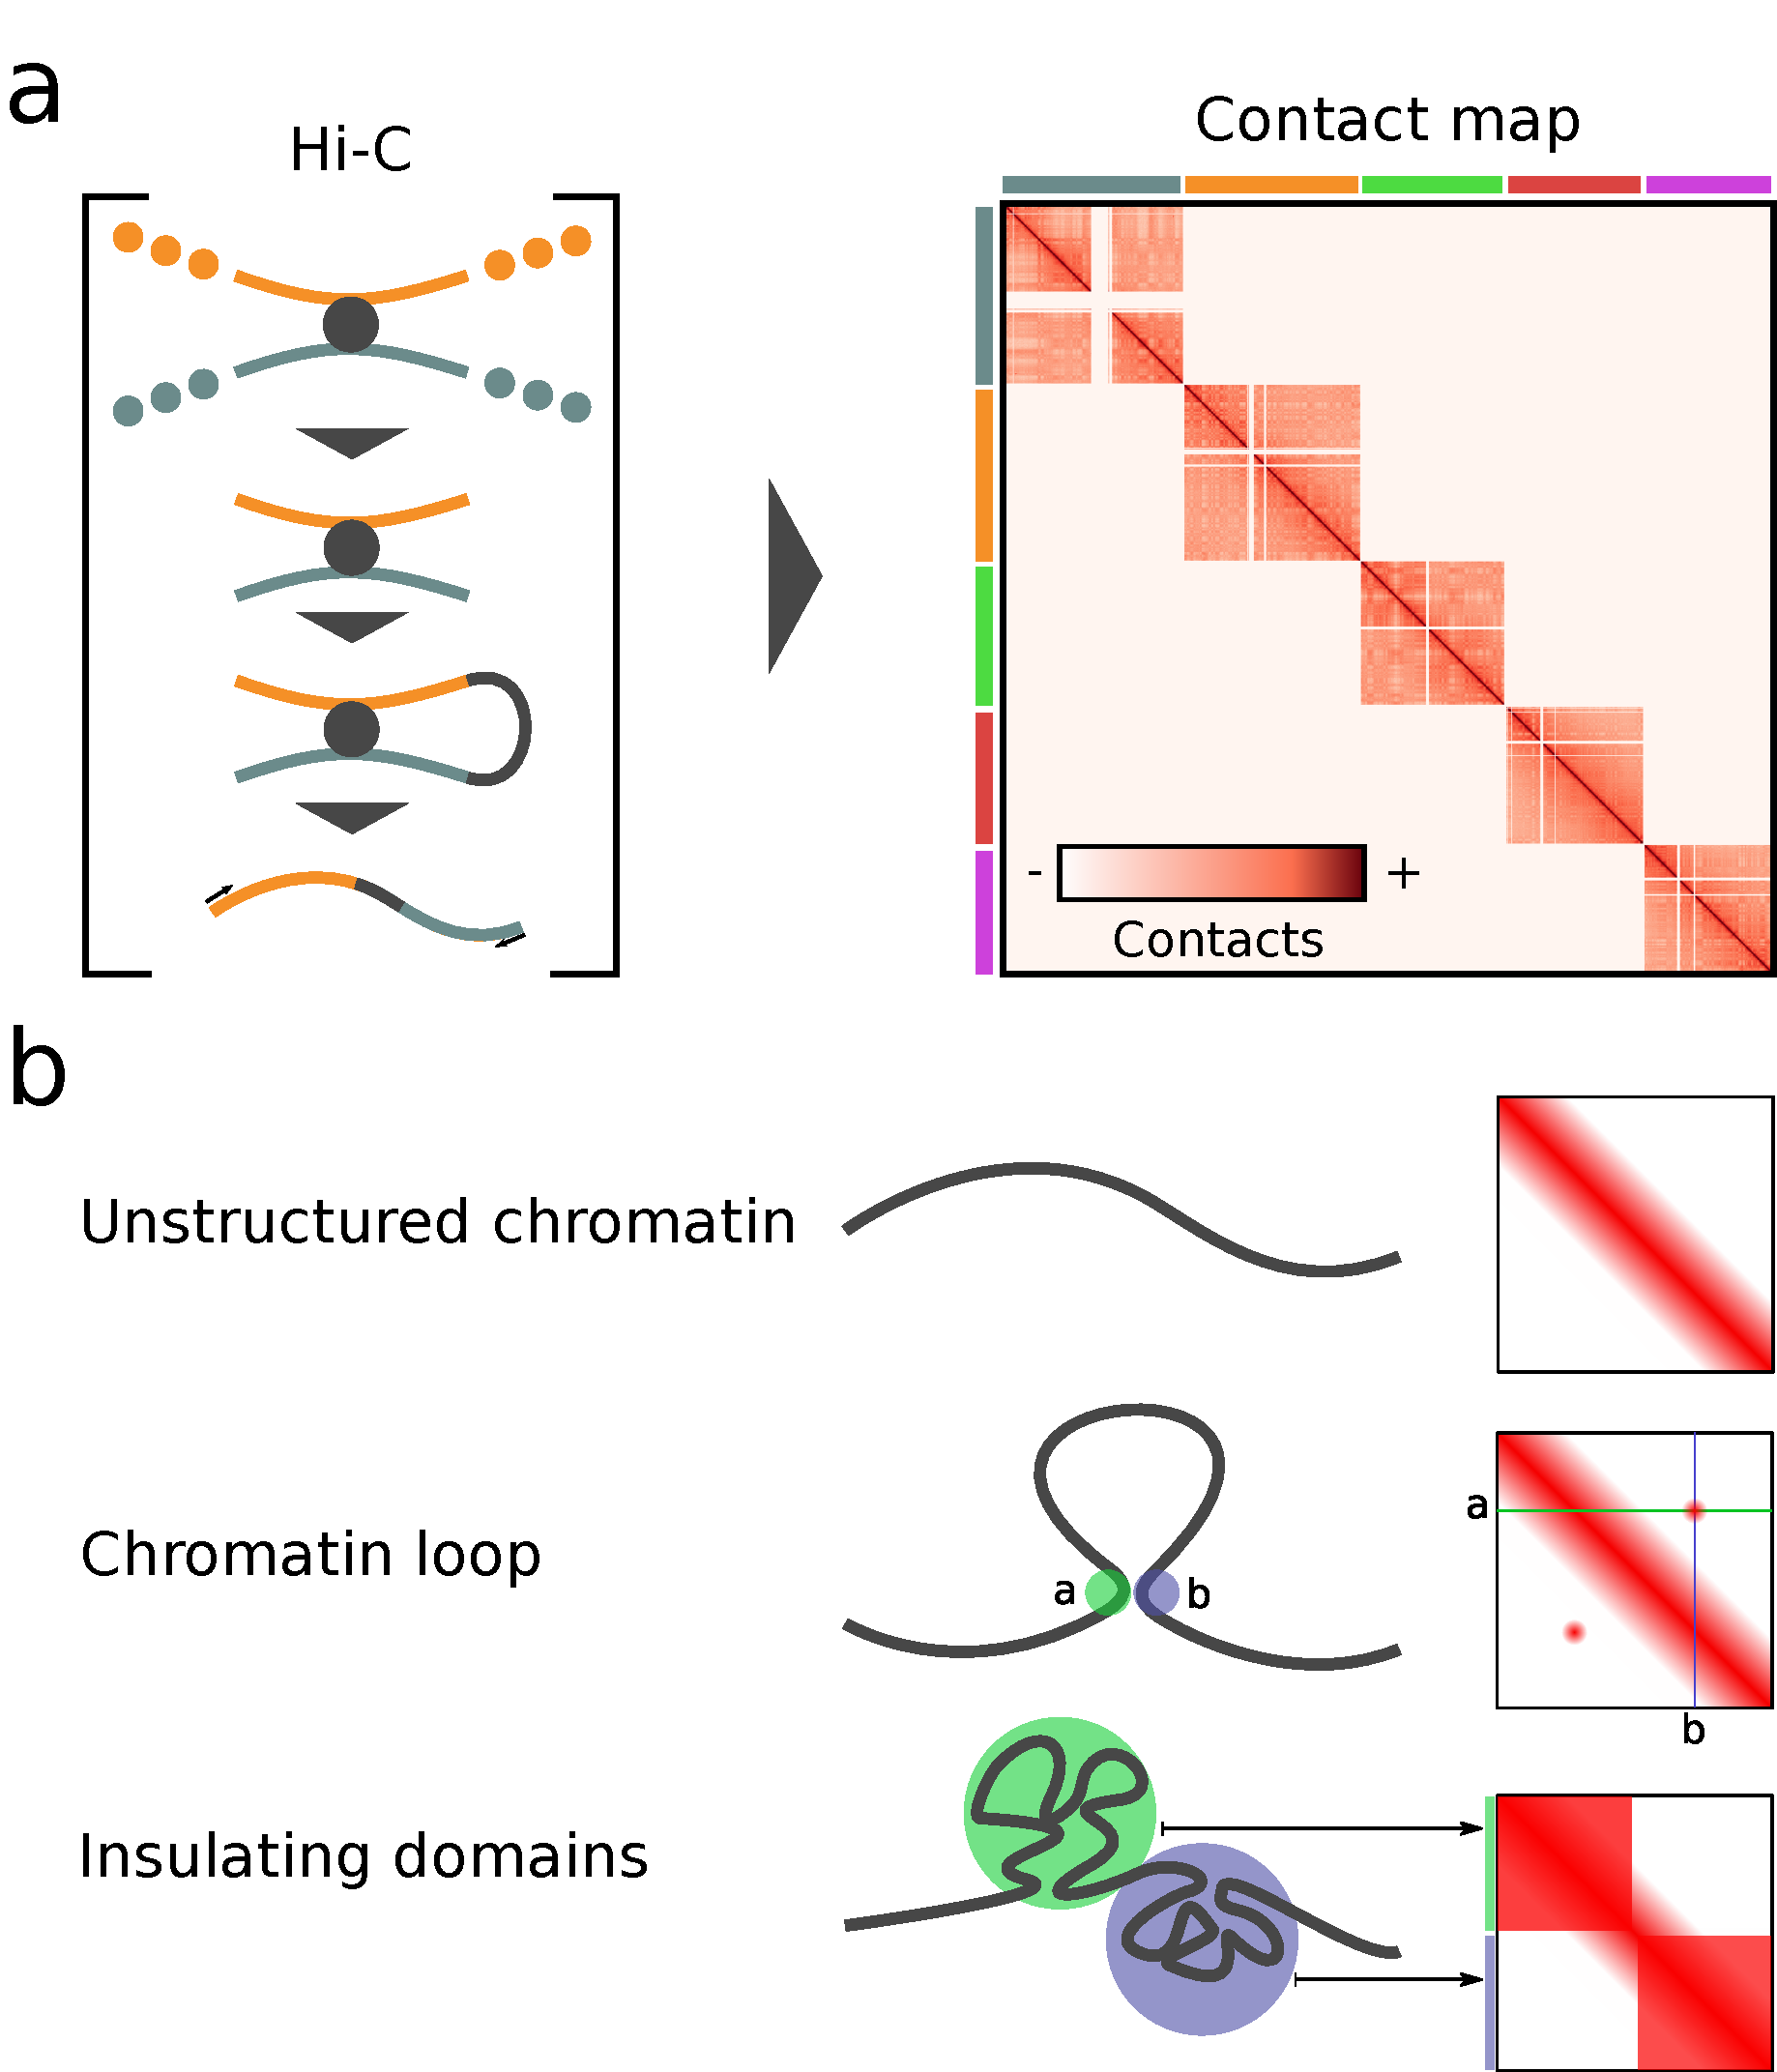
\includegraphics[width=\textwidth]{Parts/Part01/gfx/hic_interpretation.pdf}
    \caption{Interpretation of Hi-C contact maps: \textbf{a}: The Hi-C protocol (left) generates millions of read pairs representing contacts between genomic loci in a population of cells. Those contacts can be stored into an all-versus-all contact matrix (right) averaging all contacts in the population. Each chromosome in the matrix forms a square of strong self-interactions along the diagonal due to chromosomal territories. \textbf{b:} Within each chromosomal map, different contact patterns reflect specific conformations (right). The main feature of a contact map is the diagonal gradient (top) caused by the contact decay according to genomic distances. Chromatin loops between two anchor loci are visible as dots away from the diagonal (middle). Insulation domains form squares along the diagonal of a chromosome where loci within the same domain interact strongly, but interactions between domains are depleted}
	\label{fig:01-02:hic}
\end{figure}

In many eukaryotes, chromatin is also segregated into active and inactive compartments, commonly known as "euchromatin" and "heterochromatin" or A/B compartments. The A (active) compartment has higher GC content, gene density and gene expression than its counterpart \cite{lieberman-aidenComprehensiveMappingLongRange2009a}. A and B compartments also occupy separate spaces in the nucleus, whereas the A compartment is located towards the middle of the nucleus, the B compartment is relegated to the nuclear periphery and associated with lamina domains \cite{steenselLaminaAssociatedDomainsLinks2017}. This spatial segregation results in preferential physical interactions within the same compartment, which are reflected on Hi-C contact maps by a plaid-like pattern. 

\subsection{Analysis of chromosome contact maps}

The most visible element on any chromosome contact map is the diagonal gradient reflecting the power-law relationship between genomic distance and contact frequency. This is often called the distance-decay function or $P(s)$ where $s$ means genomic distance and $P$ probability of contacts. The slope of the $P(s)$ in itself holds information on the relative contribution of short range and long range contacts in the chromosome, which is linked to chromosome compaction.

Because this gradient is so strong, it often obscures other patterns that may be of interest. A common preprocessing step to account for it is to apply an \acrfull{o/e} normalization of the Hi-C map, where each pixel is divided by the average of its diagonal. It is easier to make out lower intensity patterns such as domains, compartments and chromatin loops on the resulting map.

After \acrshort{o/e} normalization, the compartment signal is generally the most salient feature on the contact maps. It can be extracted using \acrfull{PCA} on the normalized contact map \cite{lajoieHitchhikerGuideHiC2015} and retrieving the eigenvector (i.e. principal component) explaining the most variance. In some cases where compartment signal is weak (e.g. noisy datasets), a more robust approach is to select the eigenvector with the strongest absolute correlation to a separate feature, such as gene expression or GC content \cite{sergeyvenevOpen2cCooltoolsV02021}. The sign of the eigenvector is arbitrary, and it must be "phased" with the feature by flipping its sign to ensure a positive correlation with the said feature. In the phased vector, regions in the A compartment will contain positive values and \textit{vice versa}. The positions at which the sign changes are boundaries between different compartments.

\begin{figure}[htb]
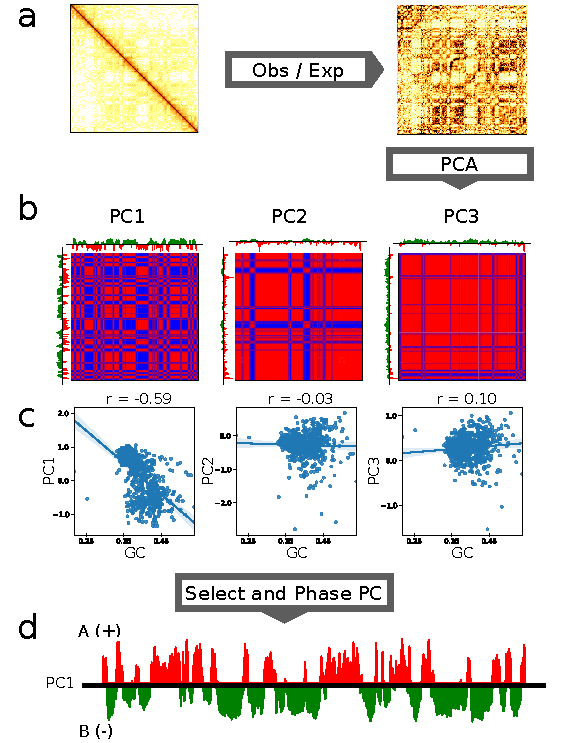
\includegraphics[width=\textwidth]{Parts/Part01/gfx/hic_pca_compartments.pdf}
\caption{Representation and analysis of chromatin compartments in Hi-C. \textbf{a:} Higher frequency of interactions within the same compartments result in a plaid-like pattern on chromosome contact maps. This organization is easier to see when applying \acrfull{o/e} normalization on the contact map. \textbf{b:} \acrfull{PCA} can extract the coordinates of A/B compartments. The first few eigenvectors are correlated with an external signal associated with active chromatin. For visualization, the outer product of each eigenvector is shown, yielding the rank-1 reconstruction of the contact map. The eigenvector with the highest correlation to the external signal is then selected and "phased" to ensure positive values represent A compartment.}
\label{fig:01-02:compartments}
\end{figure}

Another other useful vector often extracted from contact maps is the insulation score. As mentioned previously, many genomes are segmented into \acrshort{TAD}s containing frequently interacting regions, and often co-regulated genes. Regions in different \acrshort{TAD}s are insulated from each other, and the strength of this insulation can be measured at any given region as the ration of contacts across that region (upstream with downstream), relative to background on each side. Various derivatives of the insulation score have been developed and are used to detect \acrshort{TAD}s in several tools.

Some tools detect chromatin loops by looking for local enrichment of contacts, appearing as dots away from the diagonal. However, current loop detection algorithms suffer from low detection rates (recall). As such, an alternative approach is to focus on a set of genomic intervals of interest (e.g. binding sites of a transcription factor) and compute a window average of all pairs of intervals. The resulting average, often called pileup, can be used to visualize the present of chromatin loops between regions, or be compared between conditions.

In many cases, such cellular differentiation, it is useful to measure changes in Hi-C contacts between conditions. In that regard, the most global comparison, is to compute a similarity metric between pairs of samples. This is also useful as quality control, to compare technical (replicates) and biological (conditions) variability. The most commonly used methods do this using a metric based on the Pearson coefficient.

Rather than computing a single metric for each sample, an important application of Hi-C is to identify regions where the chromatin behaviour changes. Several methods aiming to achieve this are based on existing methods for RNA-seq. In this analogy, they consider each bin of the genome as a "gene" and their contacts as an expression count. They then model the bin intensity changes to identify those whose values is consistently changing between conditions across multiple replicates. This approach relies on solid statistical grounds, but it often does not address the question at hand. Often times, when analysing Hi-C data, we are interested in finding specific structures appearing or disappearing rather than a simple contact change at a region. The development of methods to discover relevant changes in chromatin conformmation is still an active area of research.

\section{Combining layers of biological informations}

The central dogma of biology - "DNA makes RNA and RNA makes protein" - exposes a linear set of reactions carrying the flow of information in living organisms. It is now known that these reactions by themselves are hardly sufficient to explain the complexity of biological processes. The fine tuning required for proper regulation is achieved through feedback loops and cross-talk between the different types of molecules (Fig. \ref{fig:01-02:central-dogma}). Common examples are methylation of DNA by proteins to reduce gene expression \cite{zemachGenomeWideEvolutionaryAnalysis2010}, noncoding RNAs recruiting proteins to repress transcription \cite{wangLongNoncodingRNA2018} or directly repressing translation by preventing ribosome binding \citep{sharmaSmallRNARegulates2007,vecerekControlFurSynthesis2007}.

\begin{figure}[htb]
    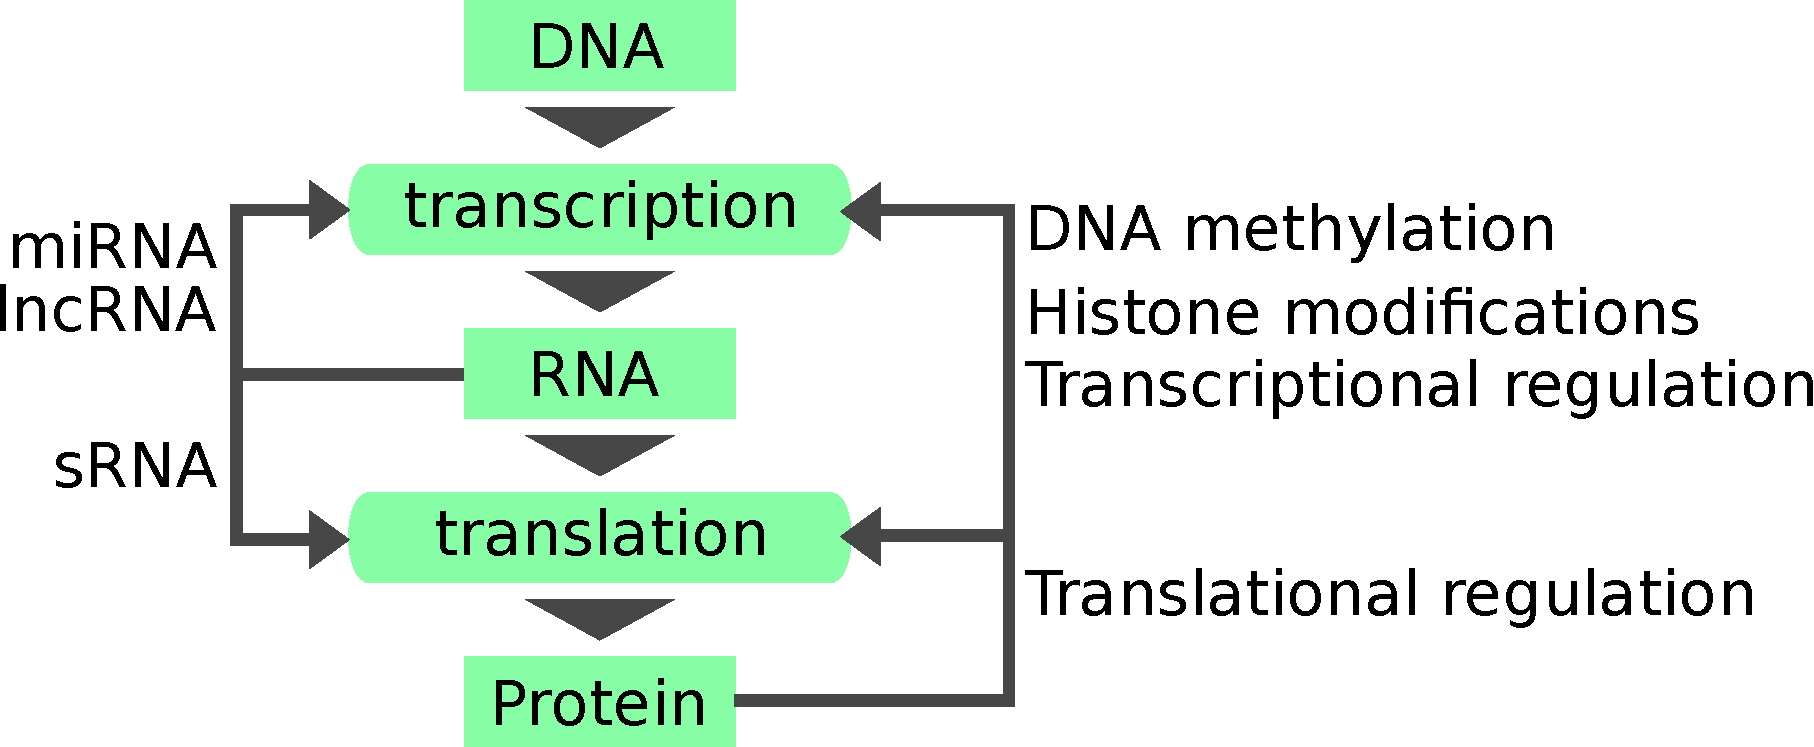
\includegraphics[width=0.8\textwidth]{Parts/Part01/gfx/central_dogma_regulation.pdf}
    \caption{Central dogma of molecular biology. Products and reactions from the central dogma are shown in green, with grey arrows showing some of the regulatory interactions between the different biomolecules.}
    \label{fig:01-02:central-dogma}
\end{figure}

There is now a growing area of research focusing on the development of methods that combine these layers of information. They aim to gain an integrative view of biology to better model the behaviour of molecular networks. This is done by combining "omics" datasets measuring various biomolecules, such as genetic mutations, gene expression, protein binding, histone modifications or protein abundance.

One of the main challenges is to find efficient ways to combine these informations to extract meaningful biological information. More often than not, they are analysed separately to find regions of deregulation common to the different layers. But there have already been attempts at fully integrating these levels of informations %MOFA, DL from Anshul Kundaje

Another challenge is the difficulty to combine different datasets due to technical heterogeneities or biological differences such as different strains or experimental conditions.
 % Chapter 2
% Chapter X

\chapter{CHAP} % Chapter title

\label{ch:01-03} % For referencing the chapter elsewhere, use \autoref{ch:name} 

%----------------------------------------------------------------------------------------

\section{SEC}

\blindtext % Chapter 3
%% Chapter X

\chapter{Thesis objectives} % Chapter title

\label{ch:01-04} % For referencing the chapter elsewhere, use \autoref{ch:name} 

Throughout this first part, we have laid out the scope of host-pathogen interactions and summarized the current state of genomics in relation to regulation and 3D genomes. Although genomics is a fast changing field, there is a need for computational tools to extract meaningful biological information from the wealth of data.

Throughout the next part, we will introduce our contributions to the field and main results. In the first chapter, we explain our methodological developments related to chromosome conformation capture technologies. In the second chapter, we will present our chromosome scale genome assembly of \textit{A. castellanii}. We then use this resource for our main findings on the genomic changes happening during infection by \textit{L. pneumophila}. Chapter 3 will focus on murine bone macrophages infection by \textit{S. enterica} and the genomic alterations it entails. Finally, in chapter 4, we will discuss additional results related to the implications of viral integrations linked to hepatocellular carcinoma in the human genome. We will end with part 3 where we discuss various aspects of genomics in infection biology, including prospects and limitations.

In this work, we develop accessible and performant methods to extract information from 3C technologies and use them to identify changes happening during infections in various organisms. We then use external data such as gene expression to assess the genes involved in those alterations and discuss how they could be associated with the infection process.
%----------------------------------------------------------------------------------------

 % Chapter 4 
\cleardoublepage % Empty page before the start of the next part
%
%%------------------------------------------------
%
\ctpartquote{\cleanchapterquote{Unfortunately, no one can be told what The Matrix is. You'll have to see it for yourself.}{Morpheus}{The Matrix}}

\ctparttext{In this second part, we present new results produced in the frame of this work. We start by describing tools and algorithms developed to address the questions at hand. In later parts, we dive into the biological results and discuss their significance.
}

\part{Results} % Second part of the thesis


% Chapter X

\chapter{CHAP} % Chapter title

\label{ch:02-01} % For referencing the chapter elsewhere, use \autoref{ch:name} 

%----------------------------------------------------------------------------------------

\section{SEC}

\blindtext % Chapter 1
% Chapter X

\chapter{Infection of \textit{Acanthamoeba castellanii} by \textit{Legionella pneumophila}} % Chapter title

\label{ch:02-02} % For referencing the chapter elsewhere, use \autoref{ch:name} 

%----------------------------------------------------------------------------------------

\section{Genome assembly}

\section{Strains comparison}

\section{Changes during infection}
 % Chapter 2
% Chapter X

\chapter{CHAP} % Chapter title

\label{ch:02-03} % For referencing the chapter elsewhere, use \autoref{ch:name} 

%----------------------------------------------------------------------------------------

\section{SEC}

\blindtext % Chapter 3
% Chapter X

\chapter{CHAP} % Chapter title

\label{ch:02-04} % For referencing the chapter elsewhere, use \autoref{ch:name} 

%----------------------------------------------------------------------------------------

\section{SEC}

\blindtext % Chapter 4
\cleardoublepage % Empty page before the start of the next part
%
%%------------------------------------------------
%
\ctpartquote{quote}
\ctparttext{\blindtext} % Text on the Part 2 page describing the content in Part 2

\part{PART} % Second part of the thesis
% Chapter X

\chapter{Biological and technical discussions} % Chapter title
\label{ch:03-01} % For referencing the chapter elsewhere, use \autoref{ch:name} 

\section{Host plasticity of intracellular bacteria}

Throughout the previous part, we have developed new approaches to detect chromatin features and quantify their changes during infection (Chap. \ref{ch:02-01}). We then applied these methods in two different infection settings: Infection of the amoeba \textit{A. castellanii} by \textit{L. pneumophila} (Chap. \ref{ch:02-02}) and of murine bone marrow macrophages by \textit{S. enterica} (Chap. \ref{ch:02-03}). Although both are intracellular bacteria with similar infection strategies, they can infect completely different hosts. The size of the mouse haploid genome outclasses that of \textit{A. castellanii} by two orders of magnitude (4.3Gbp vs 45Mbp) and its spatial organization is much more complex, with A/B compartments and intricate nested loops bridging very long distances. Despite all their differences, both unicellular and human hosts are susceptible to \textit{L. pneumophila} infection. This is most impressive knowing that human is an evolutionary dead-end for \textit{L. pneumophila} due to the absence of human-to-human transmission. The bacterial genome is therefore shaped exclusively by selective pressure in its unicellular hosts. The ability to infect multicellular hosts is probably linked to the high conservation of targeted pathways and has been attributed to the wide range of protozoan hosts infected by the bacterium \cite{molofskyDifferentiateThriveLessons2004}.

This conservation was also visible in our results, as several processes deregulated during infection are common between \textit{Legionella} and \textit{Salmonella}, such as cell cycle regulation, protein ubiquitination and transmembrane transport.

%----------------------------------------------------------------------------------------

\section{Combination of effects}

The analyses presented in this work focus on the description of changes happening in the 3D genome during infection. One issue with this type of experiments is that we observe the combined effect of the pathogen activity and the host immune response. There are means to dampen one of these effects, such as the use of mutant pathogens unable secrete effector proteins as control to trigger host response (as used in Chapter \ref{ch:02-03}). Although these controls do not completely emulate the pathogen activity, as they will not replicate  \cite{vogelConjugativeTransferVirulence1998} and therefore will not elicit the same immune response, they are still useful to separate the effect of the infection. In the case of \textit{L. pneumophila} (Chap. \ref{ch:02-02}), reproducing the infections with mutants for the dotA secretion system and romA methyl-transferase would allow to further deconvolute the chromatin changes due to the infection and romA activity from the rest.

At large scale, decoupling and deciphering the different factors at play during infection ultimately requires the use of mutagenesis screen using Transposon insertion or CRISPR. Such approaches, only assess the effect on host survival and not chromatin changes, and to our knowledge there is no method to screen for chromatin modifiers. Regardless, more descriptive approaches such as the ones used in this work are still important to understand the extent of changes happening during infection. Specifically, they can still inform us on the type of structural changes that the genome undergoes and global importance of genome organization during infection.


\section{Reproducibility and reliability challenges}

% Impact of the reproducibility crisis
Results from genomics analyses are especially sensitive to the parameters and methods used. This makes reproducibility in bioinformatics of utmost importance. Just like RNA-seq, Hi-C also has important technical variability which needs to be accounted for using multiple replicates.

It was proposed that RNA-seq experiments for differential expression analysis should comprise at least 6 replicates and ideally 12 \cite{schurchHowManyBiological2016}. While this is probably true for most omics experiments, this entails a high cost which is often the limiting factor when designing experiments in genomics.

The core issue with low replicate numbers is the impossibility to distinguish between biological variability between replicates and differences due to the condition of interest. As a consequence, when fewer replicates are used, lower effect sizes (fold changes in the case of gene expression) become undetectable. This is especially problematic when studying gene regulation, where small changes in expression could be relevant.

% Mention beyond p-values ?

% Importance of software quality and standardisation
Unlike RNAseq, where the standard for analyses is well established and most softwares are able to account for replicates and experimental design, most methods available for Hi-C analysis do not leverage replicate information. This limits the power of analysis to detect only major changes. The lack of standards for Hi-C data formats and processing also causes a general fragmentation of bioinformatic tools, with many redundant softwares of variable quality. One recurrent issue is the absence or low quality of unit tests and documentation, which are unfortunately still not regarded as standard in the computational biology community. Unit tests could be viewed as an equivalent to control experiments in molecular biology, as they validate each logic piece of the software using inputs with known truths. Software lacking these controls is more likely to have undetected bugs that could impact results and lead to false conclusion.
% The importance of standardisation

Some general practices can of course be adopted to address these issues, such as writing comprehensive documentation, solid tests and maintain software, but as it stands, there is no incentive to do so in academia. Ultimately, these directives need to be enforced globally in the peer review process by journals, so that tools need to meet quality standards to reach publication.

Although adopting such practices will increase the effort and time required to develop methods, this also means the resulting tools will be more reliable, easier to use and more widely adopted. Fortunately, recent years have seen an increasing adoption of good practices in bioinformatic software. One such example is the \textit{nf-core} ecosystem backed by SciLifeLab, a public institution dedicated to open-source scientific software development \url{https://www.scilifelab.se}. The generalization of similar initiatives could mean that the quality of academic software for bioinformatics will undergo major improvements in the forseeable future \cite{ewelsNfcoreFrameworkCommunitycurated2020}. % Chapter 1
% Chapter X

\chapter{Perspectives of genomics for infection biology} % Chapter title

\label{ch:03-02} % For referencing the chapter elsewhere, use \autoref{ch:name} 

%----------------------------------------------------------------------------------------

\section{The 3D genome and the advent of deep learning}
% Deepnog (annotation)
% DeepHiC, SRHic, ...(resolution)
% akita & deepc

\blindtext % Chapter 2
% Chapter X

\chapter{Future perspective} % Chapter title

\label{ch:03-03} % For referencing the chapter elsewhere, use \autoref{ch:name} 

As 3C protocols improve and the cost of sequencing decreases, it will be possible to probe finer details of spatial regulation during bacterial infection. While current projects are mostly limited to analyzing major changes, higher sequencing depth and increasing numbers of replicates should allow for more contrast and with it, the detection of more subtle changes in spatial interactions.

This work is still among the first of its kind and we expect to see major developments in the use of 3D genomics to understand dysregulation in infection. There is still much to be learnt in the interplay of the various layers of regulation, and spatial organization will likely become an integrative part of many projects aiming to understand it.
% Single cell (spatial heterogeneity)

%----------------------------------------------------------------------------------------
 % Chapter 3
% Chapter X

\chapter{CHAP} % Chapter title

\label{ch:03-04} % For referencing the chapter elsewhere, use \autoref{ch:name} 

%----------------------------------------------------------------------------------------

\section{SEC}

\blindtext % Chapter 4     

\cleardoublepage % Empty page before the start of the next part
%
%%------------------------------------------------
%
\ctpartquote{quote}
\ctparttext{\blindtext} % Text on the Part 2 page describing the content in Part 2

\part{PART} % Second part of the thesis
% Chapter X

\chapter{CHAP} % Chapter title

\label{ch:04-01} % For referencing the chapter elsewhere, use \autoref{ch:name} 

%----------------------------------------------------------------------------------------

\section{SEC}

\blindtext % Chapter 1
% Chapter X

\chapter{CHAP} % Chapter title

\label{ch:04-02} % For referencing the chapter elsewhere, use \autoref{ch:name} 

%----------------------------------------------------------------------------------------

\section{SEC}

\blindtext % Chapter 2
% Chapter X

\chapter{CHAP} % Chapter title

\label{ch:04-03} % For referencing the chapter elsewhere, use \autoref{ch:name} 

%----------------------------------------------------------------------------------------

\section{SEC}

\blindtext % Chapter 3
% Chapter X

\chapter{CHAP} % Chapter title

\label{ch:04-04} % For referencing the chapter elsewhere, use \autoref{ch:name} 

%----------------------------------------------------------------------------------------

\section{SEC}

\blindtext % Chapter 4      

\cleardoublepage % Empty page before the start of the next part
%
%%------------------------------------------------
%
\ctpartquote{quote}
\ctparttext{\blindtext} % Text on the Part 2 page describing the content in Part 2

\part{PART} % Second part of the thesis
% Chapter X

\chapter{CHAP} % Chapter title

\label{ch:05-01} % For referencing the chapter elsewhere, use \autoref{ch:name} 

%----------------------------------------------------------------------------------------

\section{SEC}

\blindtext % Chapter 5
\cleardoublepage % Empty page before the start of the next part

% --------------------------
% Back matter
% --------------------------
\appendix

\ctpartquote{}
\ctparttext{}
\part{Appendices}

\chapter{Supplementary information}
\label{ch:04-A:supdata}

    \section{Sparse convolution in Chromosight}
    \label{sec:04-A-01:convolution}

The explanation below describes how Chromosight reformulates convolution into a matrix multiplication problem to better handle large sparse matrices. The algorithm is inspired from \cite{NeuralNetwork2D}. For brevity, we call the operation "convolution" throughout the section, although cross-correlation could be considered more accurate as we do not transpose the kernel. Let S be the signal (Hi-C) matrix and K the kernel matrix.

\begin{equation}
    S = 
    \begin{bmatrix}
        4 & 2 & 1 \\
        2 & 4 & 1 \\
        1 & 1 & 3
    \end{bmatrix}
    K =
    \begin{bmatrix}
        10 & 12 \\
        11 & 13 \\
    \end{bmatrix}
\end{equation}

The dimensions of the desired convolution output are defined by:

\begin{equation}
    (m_S - m_K + 1) \times (n_S - n_K + 1)
\end{equation}

Note this corresponds to a convolution in "valid" mode, where edge values are truncated.

We transform each column of the kernel into a Toeplitz matrix with the same number of columns as the input signal. In this matrix, each value along the diagonals is constant.

\begin{align}
    T_0 &=
    \begin{bmatrix}
        10 & 11 & 0 \\
        0  & 10 & 11
    \end{bmatrix} &
    T_1 &=
    \begin{bmatrix}
        12 & 13 & 0 \\
        0  & 12 & 13
    \end{bmatrix}
\end{align}

The convolution of the signal and kernel can now be replaced by a sum of dot products between the signal and Toeplitz matrices built from the column filters. For each dot product, the signal is shifted according to the order of filters to respect operations performed during convolution.

\begin{align}
    C &= S * K \\
      &= S[:, 0: sn-kn+1] \cdot T_0 + S[:, 1:sn-kn+2] \cdot T_1
\end{align}

Where $\cdot$ is the matrix dot product operator and $*$ is the convolution operator.
The complete convolution algorithm used in chromosight is given as pseudocode in algorithm \ref{alg:04-B-01:convolution}.

\begin{algorithm}
\caption{Calculate $C = S * K$ using matrix products}
\label{alg:04-B-01:convolution}
\begin{algorithmic}
\REQUIRE S, $m_S \times n_S$ matrix
\REQUIRE K, $m_K \times n_K$ matrix
\ENSURE $m_S >= m_K, n_S >= n_K$
\STATE Let $\left\{T_0, ..., T_{n_K}\right\}$ be $m_K \times n_S$ matrices
\STATE $y \leftarrow 0$
\WHILE{$y \neq n_K$}
    \STATE $t \leftarrow 0$
    \WHILE{$t \neq n_S$}
        \STATE $T_y[t, :] \leftarrow K[:, t]^T$
    \ENDWHILE
\ENDWHILE
\STATE Let $C$ be a $(m_S - m_K + 1) \times (n_S - n_K + 1)$ matrix

\STATE $C \leftarrow \sum_{i=0}^{n_K}{T_{n_K} \cdot S[: , i: sn-kn+1+kj]}$ \COMMENT{Signal shifted according to each filter}
\end{algorithmic}
\end{algorithm}


\chapter{Chromosight case study}
\label{ch:04-B:demo}

\section{Quantification of metaphasic loops in yeast}
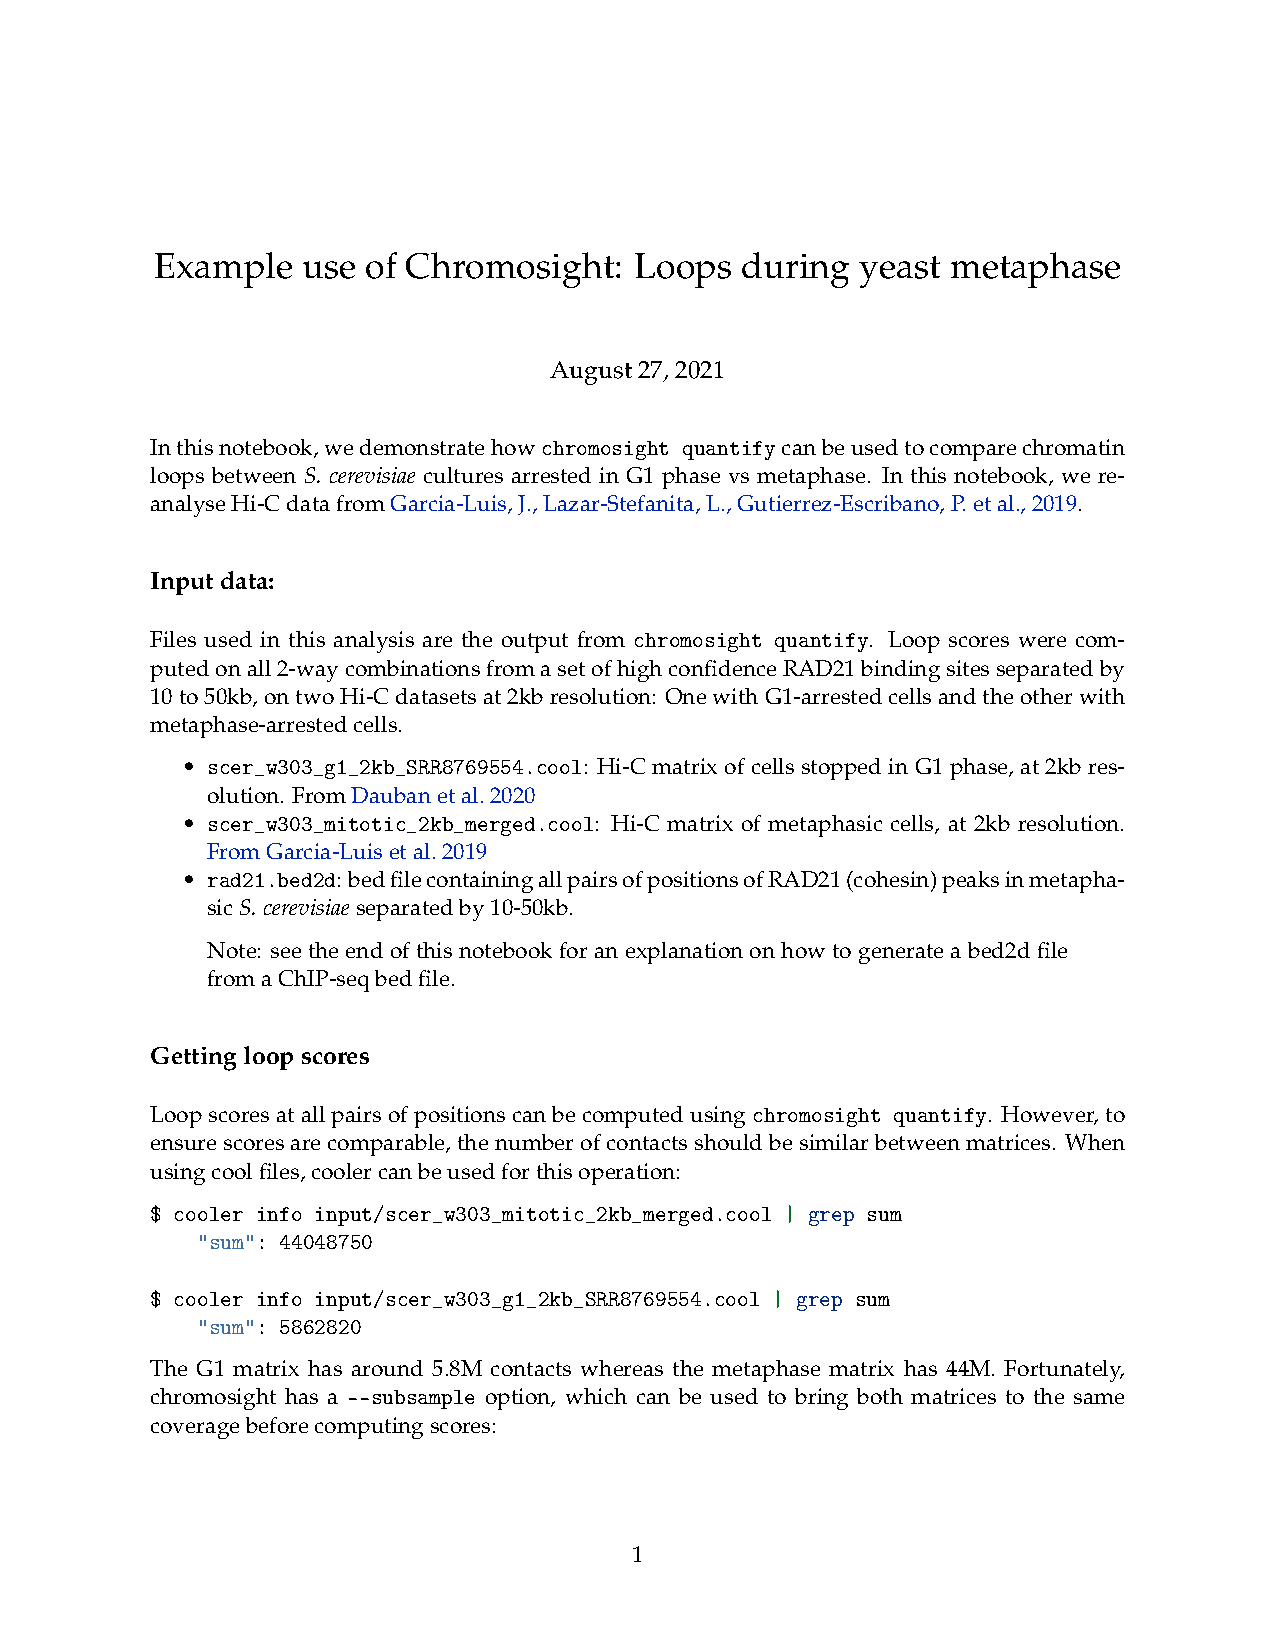
\includepdf[pages=-] {assets/g1_metaphase_yeast_example.pdf}    

\section{Output visualisation}
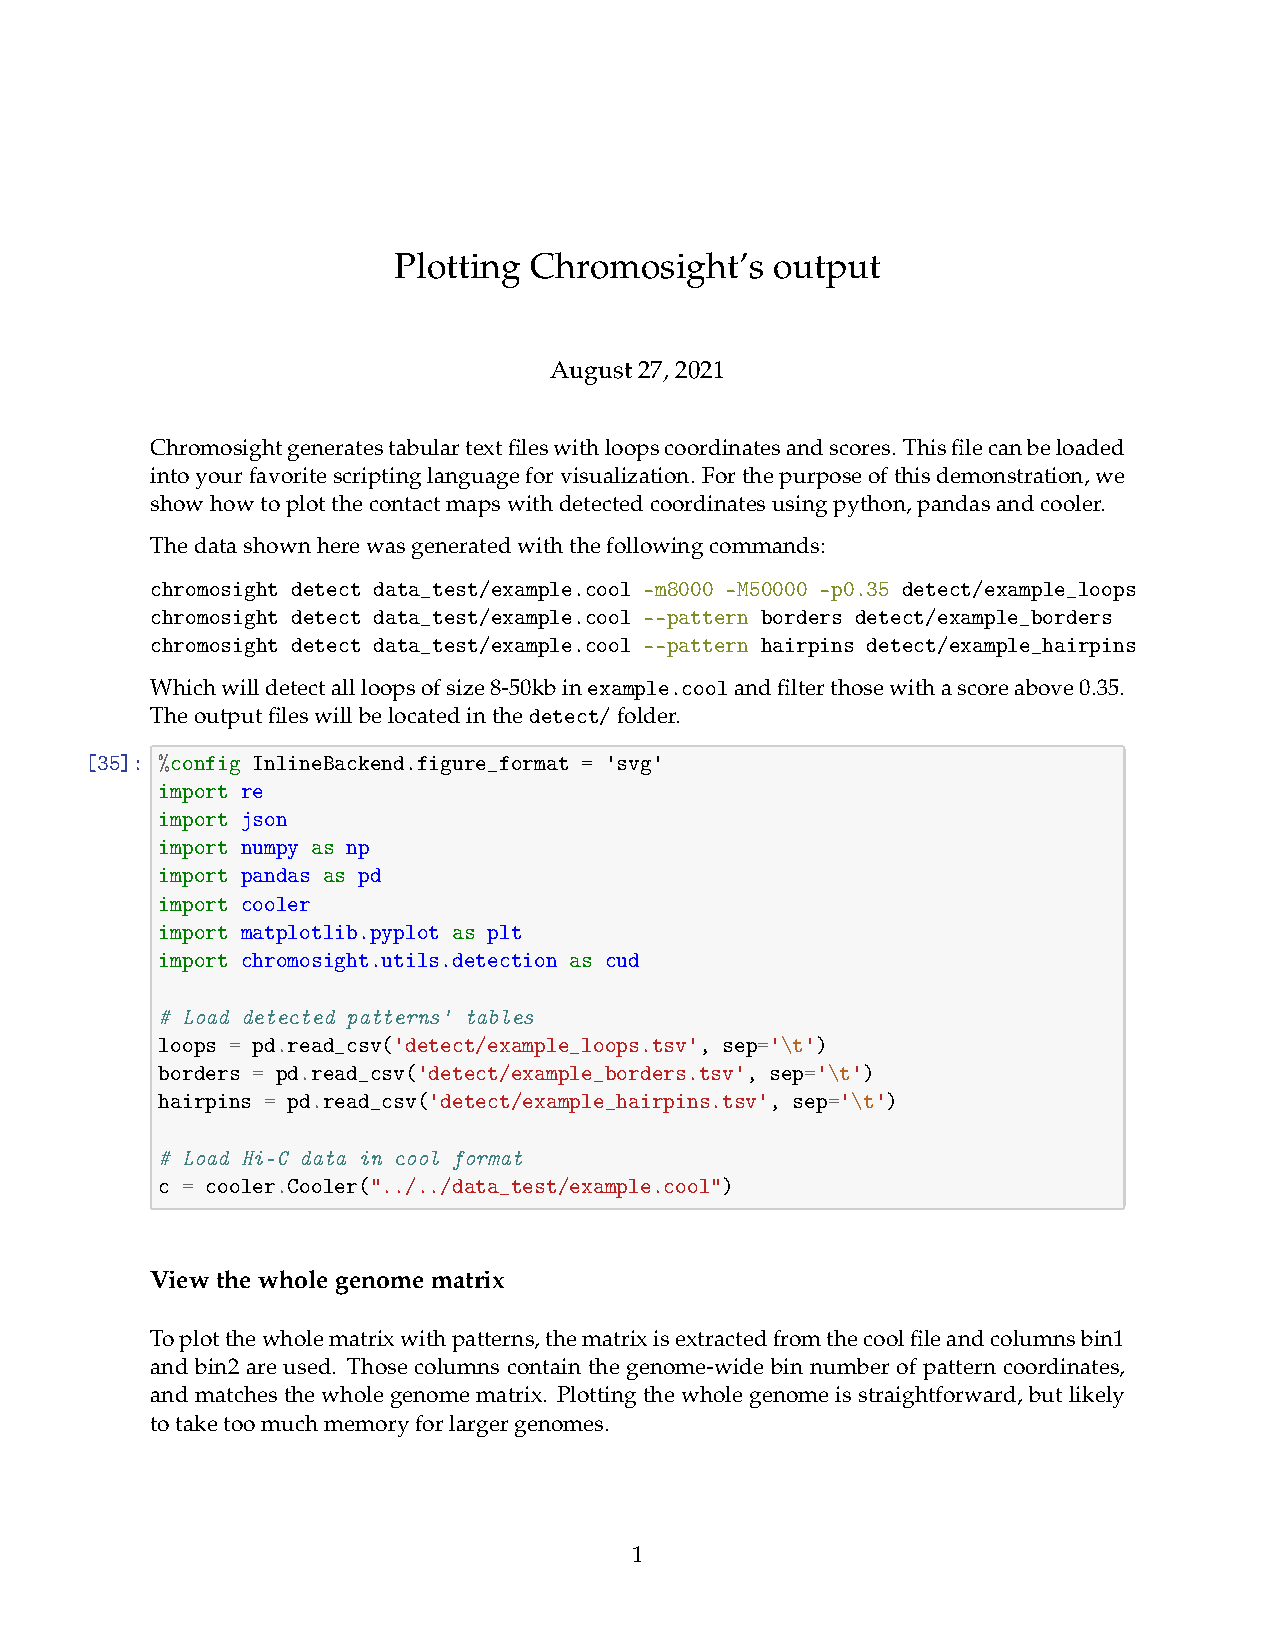
\includepdf[pages=-] {assets/plot_chromosight_output.pdf}

\chapter{Walkthrough of Pareidolia's algorithm}
\label{ch:04-C:pareidolia}

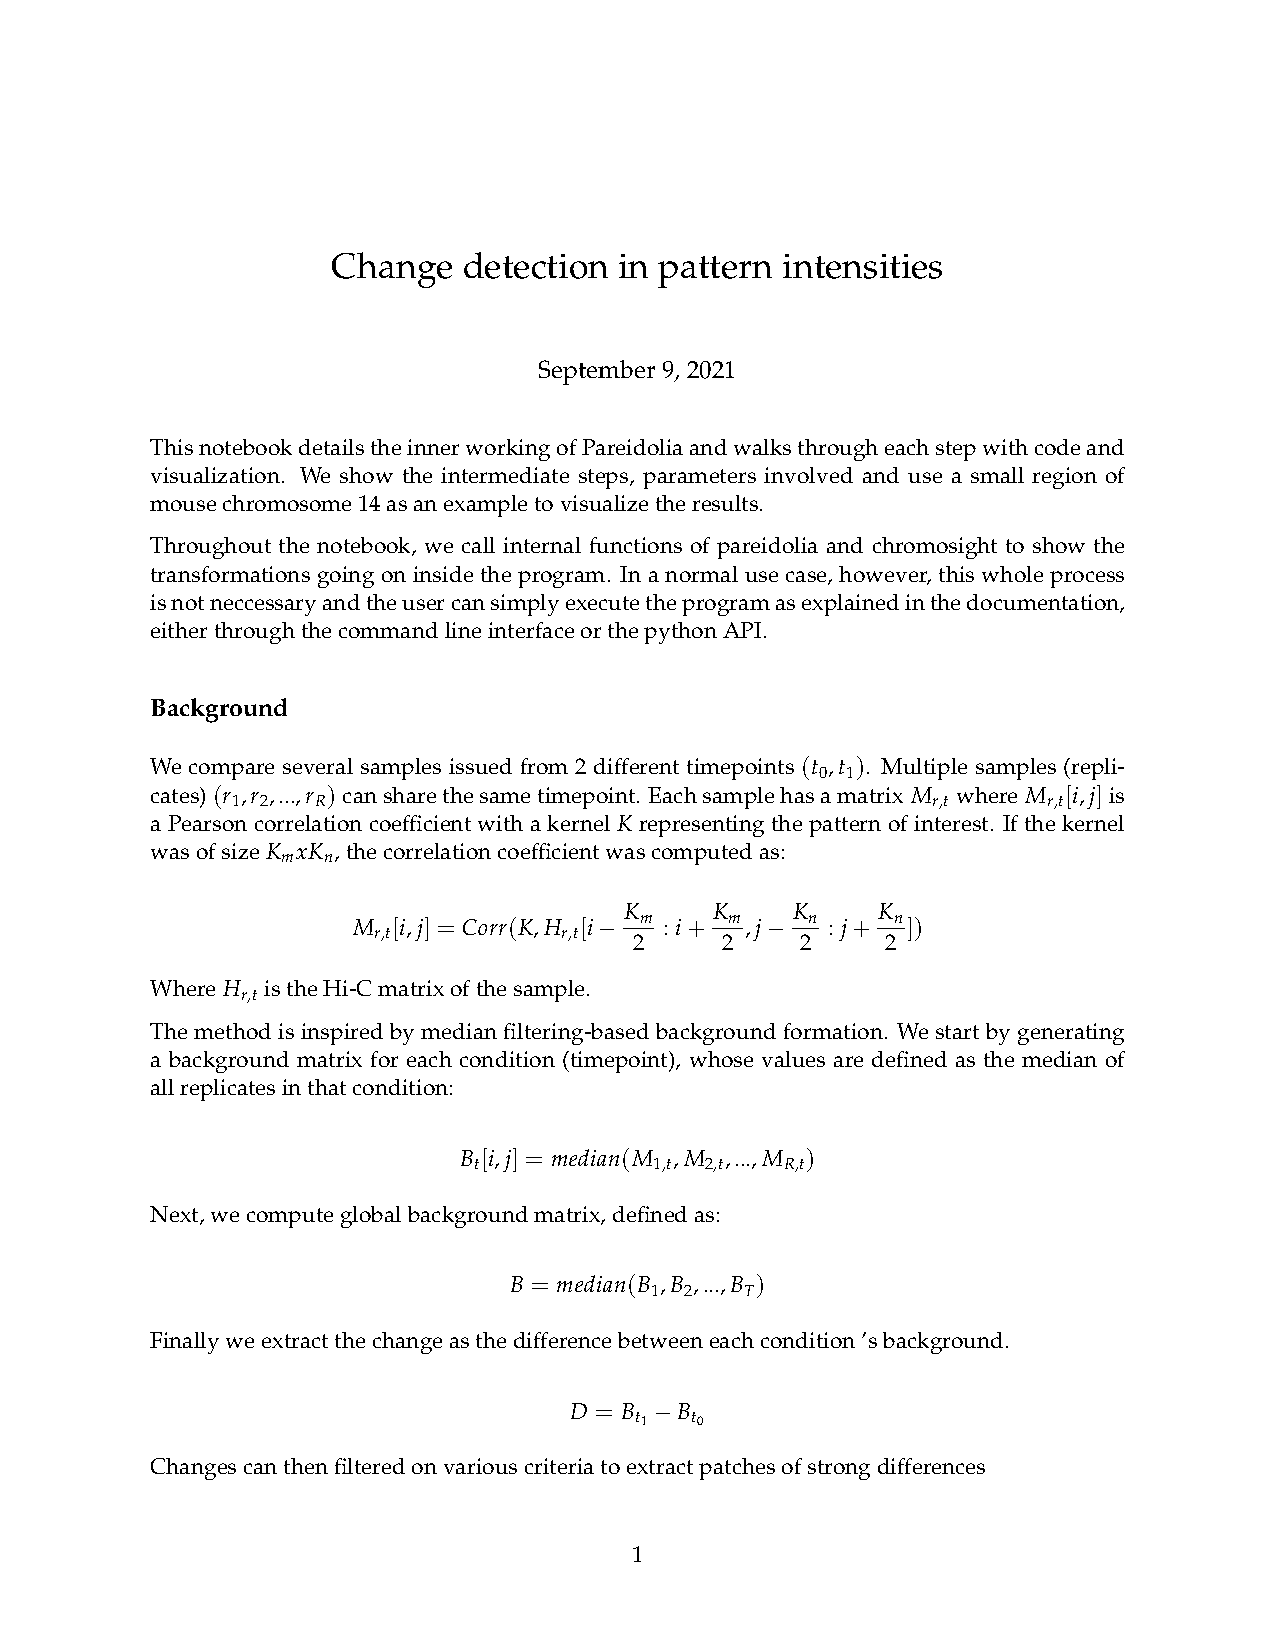
\includepdf[pages=-] {assets/pareidolia_change_detection.pdf}

%----------------------------------------------------------------------------------------
%	Glossary
%----------------------------------------------------------------------------------------
%\pagestyle{plain}
%\printglossary[type=notation]
%\clearpage

%\printglossary[type=main,style=altlist]
%\clearpage


% Bibliography
% %\renewcommand*{\bibname}{new name} % Uncomment to change the name of the bibliography
% %\setbibpreamble{} % Uncomment to include a preamble to the bibliography - some text before the reference list starts

{%
\setstretch{1.1}
\renewcommand{\bibfont}{\normalfont\small}
% \setlength{\biblabelsep}{5pt}
\setlength{\bibitemsep}{0.5\baselineskip plus 0.5\baselineskip}
\printbibliography[nottype=online,heading=bibliography]
% \printbibliography[heading=subbibliography,title={Webpages},type=online,prefixnumbers={@}]
}
\cleardoublepage

 % Publications - a page listing research articles written using content in the thesis

\pdfbookmark[1]{Publications}{Publications} % Bookmark name visible in a PDF viewer

\chapter*{Publications} % Publications page text

Some ideas and figures have appeared previously in the following publications:\\

\noindent Put your publications from the thesis here. The packages \texttt{multibib} or \texttt{bibtopic} etc. can be used to handle multiple different bibliographies in your document.

%\begin{refsection}[ownpubs]
%    \small
%    \nocite{*} % is local to to the enclosing refsection
%    \printbibliography[heading=none]
%\end{refsection}

%\emph{Attention}: This requires a separate run of \texttt{bibtex} for your \texttt{refsection}, \eg, \texttt{ClassicThesis1-blx} for this file. You might also use \texttt{biber} as the backend for \texttt{biblatex}. See also \url{http://tex.stackexchange.com/questions/128196/problem-with-refsection}. % Publications from the thesis page

% !TEX root = ../my-thesis.tex
%
\pagestyle{empty}
\hfill
\vfill
\pdfbookmark[0]{Colophon}{Colophon}
\section*{Colophon}

This thesis was typeset with \LaTeXe.
It uses the \textit{Clean Thesis} style developed by Ricardo Langner.
The design of the \textit{Clean Thesis} style is inspired by user guide documents from Apple Inc.

Download the \textit{Clean Thesis} style at \url{http://cleanthesis.der-ric.de/}.

%
% !TEX root = ../my-thesis.tex
%
%************************************************
% Declaration
%************************************************
\pdfbookmark[0]{Declaration}{Declaration}
\chapter*{Declaration}
\label{sec:declaration}
\thispagestyle{empty}

Je soussigné \thesisName~certifie que le manuscrit présenté en vue de la soutenance est le fruit d’un travail original et que toutes les sources utilisées ont été clairement indiquées.  

Je certifie, de surcroît, que je n’ai ni copié ni utilisé des idées ou des formulations tirées d’un ouvrage, article ou mémoire, en version imprimée ou électronique, sans mentionner précisément leur origine et que les citations sont expressément signalées entre guillemets (ou par une autre disposition graphique sans ambiguïté).  

Conformément à la loi, le non-respect de ces dispositions me rend passible de poursuites devant la commission disciplinaire et les tribunaux de la République française pour plagiat universitaire.


\bigskip

% \noindent\textit{\thesisUniversityCity, \thesisDate}
\noindent\textit{Fait à \thesisUniversityCity~le \thesisDate}

\smallskip

\begin{flushright}
	\begin{minipage}{5cm}
		\rule{\textwidth}{1pt}
		\centering\thesisName
	\end{minipage}
\end{flushright}

%*****************************************
%*****************************************

%\mbox{}

% **************************************************
% End of Document CONTENT
% **************************************************
\end{document}
